\documentclass[11pt,a4paper,oneside]{book}
% default
\usepackage[hmargin={1.25in,1.25in},vmargin={1.25in,1.25in}]{geometry}
% draft
%\usepackage[hmargin={1in,1in},vmargin={1in,1in}]{geometry}

\usepackage[OT1]{fontenc}
\usepackage{fontspec}
\usepackage[Greek]{ucharclasses}

\newfontfamily{\greekfont}[Scale=MatchLowercase]{cmunrm.otf}
%\setTransitionsForGreek{\begingroup\greekfont}{\endgroup}

\makeindex
\usepackage{textcomp}
\usepackage{fancyhdr}
\usepackage{makeidx}
\pagestyle{myheadings}
\fancyhf{}
\rhead[\leftmark]{thepage}

\usepackage{url}

\parindent0em
\parskip1.5ex

%%

%%%% Packages
\usepackage{acronym}
\usepackage{amsmath}
\usepackage{amsthm}
\usepackage{amsfonts}
\usepackage{amssymb}
\usepackage{xspace}
\usepackage{enumitem}
\usepackage{mathrsfs}

%%%% PGF/TikZ
\usepackage{tikz}
\usetikzlibrary{arrows,decorations,backgrounds,positioning,fit,petri}
\tikzset{
	x=0.16\linewidth,
	y=0.16\linewidth,
	>=stealth',
	bend angle=30,
	every place/.style={
		draw=black,
		minimum size=0.055\linewidth
	},
	every transition/.style={
		fill=black,
		minimum height=0.055\linewidth,
		inner xsep=0pt,
		minimum width=3pt
	}
}

%%%% Theorems
\theoremstyle{plain}
%\newtheorem{lemme}{Lemme}
%\newtheorem{prop}{Proposition}
\theoremstyle{definition}
\newtheorem{defi}{Definition}
%\theoremstyle{remark}
%\newtheorem{conv}{Convention}

%%%% Matrices
\makeatletter
\newif\if@borderstar
\def\bordermatrix{\@ifnextchar*{%
\@borderstartrue\@bordermatrix@i}{\@borderstarfalse\@bordermatrix@i*}%
}
\def\@bordermatrix@i*{\@ifnextchar[{\@bordermatrix@ii}{\@bordermatrix@ii[()]}}
\def\@bordermatrix@ii[#1]#2{%
\begingroup
\m@th\@tempdima8.75\p@\setbox\z@\vbox{%
\def\cr{\crcr\noalign{\kern 2\p@\global\let\cr\endline }}%
\ialign {$##$\hfil\kern 2\p@\kern\@tempdima & \thinspace %
\hfil $##$\hfil && \quad\hfil $##$\hfil\crcr\omit\strut %
\hfil\crcr\noalign{\kern -\baselineskip}#2\crcr\omit %
\strut\cr}}%
\setbox\tw@\vbox{\unvcopy\z@\global\setbox\@ne\lastbox}%
\setbox\tw@\hbox{\unhbox\@ne\unskip\global\setbox\@ne\lastbox}%
\setbox\tw@\hbox{%
$\kern\wd\@ne\kern -\@tempdima\left\@firstoftwo#1%
\if@borderstar\kern2pt\else\kern -\wd\@ne\fi%
\global\setbox\@ne\vbox{\box\@ne\if@borderstar\else\kern 2\p@\fi}%
\vcenter{\if@borderstar\else\kern -\ht\@ne\fi%
\unvbox\z@\kern-\if@borderstar2\fi\baselineskip}%
\if@borderstar\kern-2\@tempdima\kern2\p@\else\,\fi\right\@secondoftwo#1 $%
}\null \;\vbox{\kern\ht\@ne\box\tw@}%
\endgroup
}
\makeatother


%%%% Document specific
\newcommand{\tupleN}{\ensuremath{\mathcal{N}}\xspace}
\newcommand{\tupleS}{\ensuremath{\mathcal{S}}\xspace}
\newcommand{\marq}{\ensuremath{\mathbf{m}}\xspace}
\newcommand{\marqi}{\ensuremath{\mathbf{m}_0}\xspace}
\newcommand{\marqp}{\ensuremath{\mathbf{m'}}\xspace}
\newcommand{\marqpi}{\ensuremath{\mathbf{m'}_0}\xspace}
\newcommand{\PT}{\ensuremath{\langle P,T\rangle}\xspace}
\newcommand{\PTm}{\ensuremath{\langle P,T, \marqi\rangle}\xspace}
\newcommand{\PTP}{\ensuremath{\langle P,T,\mathbb{P}\rangle}\xspace}
\newcommand{\PTPm}{\ensuremath{\langle P,T,\mathbb{P}, \marqi\rangle}\xspace}
\newcommand{\NPT}{\ensuremath{\tupleN = \PT}\xspace}
\newcommand{\NPTm}{\ensuremath{\tupleN = \PTm}\xspace}
\newcommand{\SPTP}{\ensuremath{\tupleS = \PTP}\xspace}
\newcommand{\SPTPm}{\ensuremath{\tupleS = \PTPm}\xspace}
\newcommand{\fire}[1]{\stackrel{#1}{\to}}
\newcommand{\firev}[1]{\stackrel{#1}{\to}_v}
\newcommand{\matI}{\mathbf{I}}
\newcommand{\matO}{\mathbf{O}}
\newcommand{\matIN}{\matI_\tupleN}
\newcommand{\matON}{\matO_\tupleN}
\newcommand{\matIS}{\matI_\tupleS}
\newcommand{\matOS}{\matO_\tupleS}
\newcommand{\Ecov}{\ensuremath{\mathscr{E}\text{-cov}}\xspace}
\newcommand{\Ucov}{\ensuremath{\mathscr{U}\text{-cov}}\xspace}
% prec pleq npleq
\newcommand{\pleq}{\preccurlyeq}
\newcommand{\npleq}{\npreccurlyeq}

%%%% Layout
\setlist[itemize]{noitemsep,nolistsep}
%\makeatletter
%\parindent 10pt
%\topsep 4pt plus 1pt minus 2pt
%\partopsep 1pt plus 0.5pt minus 0.5pt
%\itemsep 2pt plus 1pt minus 0.5pt
%\parsep 2pt plus 1pt minus 0.5pt
%
%\leftmargin 10pt \leftmargini\leftmargin \leftmarginii 10pt
%\leftmarginiii 5pt \leftmarginiv 5pt \leftmarginv 5pt \leftmarginvi 5pt
%\labelwidth\leftmargini\advance\labelwidth-\labelsep \labelsep 5pt
%
%\def\@listi{\leftmargin\leftmargini}
%\def\@listii{\leftmargin\leftmarginii
%   \labelwidth\leftmarginii\advance\labelwidth-\labelsep
%   \topsep 2pt plus 1pt minus 0.5pt
%   \parsep 1pt plus 0.5pt minus 0.5pt
%   \itemsep \parsep}
%\def\@listiii{\leftmargin\leftmarginiii
%    \labelwidth\leftmarginiii\advance\labelwidth-\labelsep
%    \topsep 1pt plus 0.5pt minus 0.5pt
%    \parsep \z@ \partopsep 0.5pt plus 0pt minus 0.5pt
%    \itemsep \topsep}
%\def\@listiv{\leftmargin\leftmarginiv
%     \labelwidth\leftmarginiv\advance\labelwidth-\labelsep}
%\def\@listv{\leftmargin\leftmarginv
%     \labelwidth\leftmarginv\advance\labelwidth-\labelsep}
%\def\@listvi{\leftmargin\leftmarginvi
%     \labelwidth\leftmarginvi\advance\labelwidth-\labelsep}
%
%\abovedisplayskip 7pt plus2pt minus5pt%
%\belowdisplayskip \abovedisplayskip
%\abovedisplayshortskip  0pt plus3pt%
%\belowdisplayshortskip  4pt plus3pt minus3pt%
%\makeatother


%%%% TMP
\newcommand{\todo}[1]{[TODO: #1]}


\begin{document}

\frontmatter
\begin{titlepage}
\begin{center}
\textbf{UNIVERSIT\'E LIBRE DE BRUXELLES}\\
\textbf{Faculté des Sciences}\\
\textbf{Département d'Informatique}
\vfill{}\vfill{}

{\Huge  The Coverability problem \vspace*{.5cm}  \linebreak[4] for parametric Petri nets}

{\Huge \par}
\begin{center}{\LARGE Alexis Reynouard}\end{center}{\Huge \par}
\vfill{}\vfill{}
\begin{flushright}{\large \textbf{Promotor :} Prof. Gilles Geeraerts}\hfill{}{\large Master Thesis in Computer Sciences}\\
{\large }\hfill{}{}\end{flushright}{\large\par}
\vfill{}\vfill{}\enlargethispage{3cm}
\textbf{Academic year 2018~-~2019}
\end{center}
\end{titlepage}
\newpage
\thispagestyle{empty} 
\null

\newenvironment{vcenterpage}
{\newpage\thispagestyle{empty} 
\vspace*{\fill}}
{\vspace*{\fill}\par\pagebreak}

%\begin{vcenterpage}
%\begin{flushright}
%    \large\em\null\vskip1in 
%    You may want\\
%   to write a dedication here\vfill
%  \end{flushright}
%\end{vcenterpage}
%\thispagestyle{empty}
%\vspace*{5cm}
%
%\begin{quotation}
%\noindent ``\emph{You may also include one or more general quotes related to your topic.}''
%\begin{flushright}\textbf{Name of the author, date}\end{flushright}
%\end{quotation}
%
%\medskip
%
%\begin{quotation}
%\noindent ``\emph{Another quote.}''
%\begin{flushright}\textbf{Name of the author, date}\end{flushright}
%\end{quotation}
%\chapter*{Acknowledgment}
%\thispagestyle{empty} 
%
%\noindent I want to thank ...

\thispagestyle{empty} 
\setcounter{page}{0}
\tableofcontents

\acrodef{PN}{Petri net}
\acrodef{PPN}{parametric Petri net}

\mainmatter
\setcounter{page}{1}

\chapter{Introduction}
\acp{PN} are a mathematical and graphical model introduced by Carl Adam Petri in 1962 \citep{Petri62,Petri66}.
It was successfully used to analyse systems in a wide range of domains, and has proven to be particularly successful for the formal verification of asynchronous systems.

In their standard definition, \acp{PN} are instantiated through many natural numbers\footnote{\lang{i.e.} a \ac{PN} may be represented as a pair of matrices whose the values are from $\naturals$.} which may represent, for example, the amount of resource needed for a given action to be carried out.

The introduction of parameters into the model to avoid the need to state these values explicitly%
\footnote{One can find in the literature many other way to use parameters in \acp{PN}. For example, place and~/~or transitions may also be parameters in order to dynamically change the network structure, like in \cite{Christensen97}.}
may have several benefits:
it may allow performing analysis of a whole family of \acp{PN} efficiently, like in \cite{Abdulla13}, or to model dynamic changes in the system, as introduced by \cite{Badouel99} as a subclass of reconfigurable nets.

The use of parameters increases the modelling power of \acp{PN} but also make some basic coverability problems undecidable in the general case \cite{David17}.

We adopt the parametric Petri net model introduced by \cite{David17}, which seems the most general, and we study the existing results and algorithms for plain Petri nets to find out whether they still hold or how to adapt them to the parametric model.

The rest of the document is as follows:
In this first part, we define the plain Petri net model (\lang{i.e.} the classical one) and the parametric model.
We then briefly motivate our study, \todo{give concrete examples of applications,} and give an overview of the previous works on parametrisation of \acp{PN}.
Finally, we place the \ac{PN} model in a broader model family: the \acp{WSTS}.\\
In a second part, we recall, first, the classical results that we will study on this new model, second, the results already obtained for the parametrized Petri net model as we have defined them.\\
Then, we focus on the parametric Petri net model to establish whether the results related to the coverability problem in the plain Petri net model still hold or if the algorithms may be adapted to this new model.

\acresetall

\todo{contributions}
% vim: set spell spelllang=en :

\section{Definitions}
\begin{defi}[\acl{PN}]
  A \acf{PN} \tupleN is a weighted oriented bipartite graph, whose the two subsets of vertices define a tuple \PT where:
  \begin{itemize}
    \item $P$ is a finite set of places,
    \item $T$ is a finite set of transitions.
  \end{itemize}
  For each transition $t \in T$ are defined (exactly) these two functions:
  \begin{itemize}
    \item $I_t : P \mapsto \mathbb{N}$ associates to each place the weight of the edge to $t$ \emph{(input weight)},
    \item $O_t : P \mapsto \mathbb{N}$ associates to each place the weight of the edge from $t$ \emph{(output weight)}.
  \end{itemize}
  It is denoted by $t = \langle I_t, O_t \rangle$.
  Because these functions define the edges of the graph, a \ac{PN} is completely defined by the tuple \PT and so is denoted by \NPT.
\end{defi}

\begin{defi}[marking]
  Given a set of place $P$, a marking over $P$ is a function $\marq : P \mapsto \mathbb{N}$ that associates $\marq(p)$ tokens to each place $p \in P$.
\end{defi}

An order on the markings is essential for the analysis of \acp{PN}. The order we will define is a well quasi order and a partial order.

\begin{defi}[quasi order]
  A quasi order on a set $\mathcal{E}$ is a binary relation $R$ that is:
  \begin{align*}
    \text{reflexive: } &&\forall x \in \mathcal{E},\ & x \mathrel{R} x \\
    \text{transitive: } &&\forall (x, y, z) \in \mathcal{E}^3,\ & (x \mathrel{R} y\land y \mathrel{R} z)\Rightarrow x \mathrel{R} z
  \end{align*}
\end{defi}

\begin{defi}[well quasi order]
  A well quasi order $\sqsubseteq$ on a set $\mathcal{E}$ is a quasi order on $\mathcal{E}$ such that, for any infinite sequence $s = e_0, e_1, e_2, \dots$ of elements from $\mathcal{E}$, there exist indices $i < j$ with $e_i \sqsubseteq e_j$. That is, there is no infinite antichain in $\mathcal{E}$ for this relation.
\end{defi}

\begin{defi}[partial order]
  A partial order on a set $\mathcal{E}$ is a quasi order $R$ that is
  \begin{align*}
    \text{antisymmetric: } &&\forall (x, y) \in \mathcal{E}^2,\ & (x \mathrel{R} y\land y \mathrel{R} x)\Rightarrow x = y
  \end{align*}
\end{defi}

\begin{defi}[partial order \(\pleq\) on the markings]
  Given a set of places $P$, the partial order \(\pleq \subseteq \mathbb{N}^{|P|} \times \mathbb{N}^{|P|}\) is such that for all pair of markings \((\marq_1, \marq_2) \in \mathbb{N}^{|P|} \times \mathbb{N}^{|P|}\) we have that \(\marq_1 \pleq \marq_2\) if and only if for all place \(p \in P : \marq_1(p) \leq \marq_2(p)\).
\end{defi}

\(\marq \prec \marqp\) denote that \(\marq \pleq \marqp \text{ and } \marqp \npleq \marq\).

\begin{lemm}[\cite{Dickson13}]
  \label{lemm:wqo}
  $\pleq$ is a well quasi order.
\end{lemm}

The following result will be useful in the sequel.

\begin{lemm}[\cite{Brams83}]
  The \ac{PN} model is \emph{strongly monotonic with regard to $\pleq$}. That is, for all \ac{PN} $\tupleN = \PTm$, for all transition $t \in T$ and for all markings $\marq_1, \marq_2, \marq_3$ of \tupleN such that $\marq_1 \prec \marq_2$ and $\marq_1 \fire{t} \marq_3$, there exists a marking $\marq_4$ of \tupleN such that $\marq_2 \fire{t} \marq_4$ and $\marq_3 \prec \marq_4$. 
\end{lemm}

In this work we will focus on an extension of the \ac{PN} model, the \ac{PPN} model, that is extended thanks to the use of parameters as input and output weights.

\begin{defi}[\acl{PPN}]
  A \acf{PPN} \SPTP is a weighted oriented bipartite graph with a finite set $\mathbb{P}$ of parameters. The two subsets of vertices are:
  \begin{itemize}
    \item $P$: a finite set of places,
    \item $T$: a finite set of transitions,
  \end{itemize}
  For each transition $t \in T$ are defined the following functions:
  \begin{itemize}
    \item $I_t : P \mapsto \mathbb{N} \cup \mathbb{P}$ associates to each place the weight of the edge to $t$ \emph{(input weight)},
    \item $O_t : P \mapsto \mathbb{N} \cup \mathbb{P}$ associates to each place the weight of the edge from $t$ \emph{(output weight)}.
  \end{itemize}
\end{defi}

As for plain \acp{PN}, this is denoted $t = \langle I_t, O_t \rangle$.

\begin{defi}[parametric marking]
  Given a set of place $P$, a parametric marking over $P$ is a function $\marq : P \mapsto \mathbb{N} \cup \mathbb{P} $ that associates $\marq(p)$ tokens to each place $p \in P$.
\end{defi}

A marking of a \ac{PN} \NPT is a marking over $P$.
A marking of a \ac{PPN} \SPTP is a \emph{parametric} marking over $P$.
Note that a marking \marq is a parametric marking where $\marq(p) \in \mathbb{N}$ for all $p \in P$.

\begin{defi}[initialized (parametric) \ac{PN}]
  An initialized \ac{PN} \NPTm (resp. \ac{PPN} \SPTPm) is a \ac{PN} (resp. \ac{PPN}) with an initial marking \marqi.
\end{defi}

This is sometimes called a \emph{marked (parametric) \ac{PN}}.
We will often refer to an initialized (parametric) \ac{PN} loosely as a (parametric) \ac{PN}.

The figure~\ref{fig:parametric-petri-net-example} shows an example of \ac{PPN} whose $\mathbb{P} = \{a, b\}$ and with an initial marking \marqi such that $\marqi(p_1) = 1$, $\marqi(p_2) = a$ and $\marqi(p_3) = 0$. The circles represent the places, the rectangles are the transitions and the dots are the tokens. If the number of token at a given place is parametric (\lang{i.e.} depends on a parameter of $\mathbb{P}$), it is written inside the circle. An arrow from a place $p$ and to a transition $t$ denotes that $I_t(p) = 1$. If there is no arrow from $p$ to $t$, $I_t(p) = 0$. If $I_t(p) \notin \{0, 1\}$, a label with the value of $I_t(p)$ is added to the arrow.
Symmetrically, the arrows from the transitions to the places indicate the output weights.

\begin{figure}[h]
  \centering
  \center
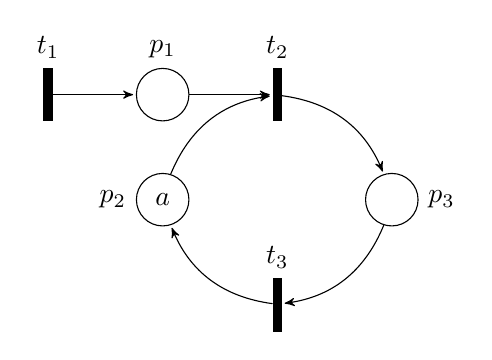
\begin{tikzpicture}[auto,x=0.12\linewidth,y=0.11\linewidth]
	\node [place] (d) [label=$p_1$] at (4,2) {};
	\node [place] (l) [label=west:$p_2$] at (4,1) {$a$};
	\node [place] (o) [label=east:$p_3$] at (6,1) {};
	
	\node [transition] (S) [label=$t_1$] at (3,2) {}
	edge [post] (d);
	\node [transition] (C) [label=$t_2$] at (5,2) {}
	edge [pre]  (d)
	edge [pre,  bend right] (l)
	edge [post, bend left]  (o);
	\node [transition] (F) [label=$t_3$] at (5,0) {}
	edge [pre,  bend right] (o)
	edge [post, bend left]  (l);
\end{tikzpicture}
\par

  \par
  \caption{An initialized \ac{PPN}}
  \label{fig:parametric-petri-net-example}
\end{figure}

We usually set an order on the places.
This allows to view the markings as vectors (here, \marqi is the column vector $(1, a, 0)^T$, where $\cdot^T$ is the transpose operator) as well as the $I$ and $O$ functions.
Likewise, we define an order on the transitions.
Therefore, $I_t$ and $O_t$ denote respectively the $I$ and $O$ functions defined for the $t$\textsuperscript{th} transition (here, $I_1 = (0, 0, 0)^T$ and $O_1 = (b, 0, 0)^T$).
Given a \ac{PPN} \SPTP, the backward and forward incidence matrices $\matIS \in (\mathbb{N} \cup \mathbb{P})^{|P|\times|T|}$ and $\matOS \in (\mathbb{N} \cup \mathbb{P})^{|P|\times|T|}$ are naturally defined by $\matIS(p, t) = I_t(p)$ and $\matOS(p, t) = O_t(p)$.
($\tupleS$ is omitted when it is obvious from the context.)
%In addition, it makes the equivalence between \acp{PN} and \emph{vector addition systems} introduced in \cite{Karp69} more explicit and
This allows to use linear algebra to analyse \acp{PN}.

\begin{figure}[h]
	\[
		\matI = \bordermatrix[{[]}]{%
					& t_1 & t_2 & t_3 \cr
			p_1 & 0   & 1   & 0   \cr
			p_2 & 0   & 1   & 0   \cr
			p_3 & 0   & 0   & 1   }
		\mspace{56mu}
		\matO = \bordermatrix[{[]}]{%
					& t_1 & t_2 & t_3 \cr
			p_1 & b   & 0   & 0   \cr
			p_2 & 0   & 0   & 1   \cr
			p_3 & 0   & 1   & 0   }
	\]
  \caption{The incidence matrices of the \ac{PN} from figure \ref{fig:parametric-petri-net-example}}
  \label{fig:incidence-matrices-example}
\end{figure}

%\begin{defi}[Vector addition system]
%  A vector addition system of dimension $n$ is a pair $\langle d, W\rangle$ where $d \in \mathbb{N}^n$ is called the \emph{start vector} and $W$ is a finite set of vector $\mathbb{Z}^n$.
%\end{defi}
%This corresponds to the definition of an initialized \ac{PN} and \todo{we will see that the semantic corresponds too}.

\subsection{Operational semantic of \acp{PN}}

Given a \ac{PN} \NPT and a marking \marq on \tupleN, a transition $t \in T$ is said \emph{enabled} by \marq if $\forall p \in P : \marq(p) \geq I_t(p)$. An enabled transition can be \emph{fired} to produce a new marking \marqp such that $\forall p \in P : \marqp(p) = \marq(p) - I_t(p) + O_t(p)$. This is denoted by $\marq \fire{t} \marqp$.
It is important to note that the effect of a transition is to add or remove a constant number of tokens at each place and does not depend on the marking from which it is fired. A \ac{PN} transition is said to have a \emph{constant effect}.
\todo{Note difference when talking about {\textomega}-Petri nets}

Here are some additional notations:
\begin{itemize}
  \item $\marq \rightarrow \marqp$ denotes that there exists $t \in T$ such that $\marq \fire{t} \marqp$.
  \item $\marq \fire{\sigma} \marqp$ where $\sigma$ is a sequence of transitions $\sigma = (t_1, \dots, t_{n-1}), t_i \in T, i \in \{1, \dots, n-1\}$ denotes that there exists a sequence of markings $\marq_1, \dots, \marq_n$ such that : $\marq = \marq_1 \fire{t_1} \cdots \fire{t_{n-1}} \marq_n = \marqp$.
  \item $\marq \fire{*} \marqp$ denotes that there exists a sequence of transition $\sigma$ such that $\marq \fire{\sigma} \marqp$.
    Note that the $\fire{*}$ relation is the reflexive and transitive closure of the relation $\rightarrow$.
\end{itemize}

\begin{defi}
  Given an \ac{PN} \NPT and a marking \marq of \tupleN:
  \begin{itemize}
    \item $\Post(\marq) = \{\marqp \mid \marq \rightarrow \marqp\}$ is the set of one-step successors of \marq,
    \item $\Pre(\marq) = \{\marqp \mid \marqp \rightarrow \marq\}$ is the set of one-step predecessors of \marq,
    \item $\Post^*(\marq) = \{\marqp \mid \marq \fire{*} \marqp\}$ is the set of successors of \marq, in any number of step.
      With $\marqi$ the initial marking of \tupleN, $\Post^*(\marqi)$ is the \emph{reachability set} of \tupleN.
    \item $\Pre^*(\marq) = \{\marqp \mid \marqp \fire{*} \marq\}$ is the set of predecessors of \marq, in any number of step.
  \end{itemize}
\end{defi}

These operators are naturally extended to sets of markings as the union of the sets obtained by applying the operator on each marking of the sets.
That is, with $M$ a set of markings of \NPT,
$\Post(M) = \{\marqp \mid \exists \marq \in M : \marq \rightarrow \marqp\}$.

For example, regarding the \ac{PPN} shown on figure \ref{fig:parametric-petri-net-example},
$\Post((0,1,0)) = \{(b, 1, 0)\}$
and
$\Post^*((0,1,0)) = \{(i, 1, 0) \mid i \in \mathbb{N}\} \cup \{(i, 0, 1) \mid i \in \mathbb{N}\}$.

All of this applies to \ac{PPN} through valuations of the parameters:
\begin{defi}[Instantiation of \acp{PPN}]
  Let \SPTPm be a \ac{PPN} and $v : \mathbb{P} \mapsto \mathbb{N}$ be a \emph{valuation} on $\mathbb{P}$.
  Then $v(\tupleS)$ is defined as the \ac{PN} obtained by replacing each parameter $a \in \mathbb{P}$ by $v(a)$.
  Thus, we have $v(\tupleS) = \langle P, T, \marqpi\rangle$ such that :
  \begin{itemize}
    \item $\matI_{v(\tupleS)}(p, t) =
      \begin{cases}
        \phantom{v(}\matIS(p, t) & \text{if } \matIS(p, t) \in \mathbb{N} \\
                 v(\matIS(p, t)) & \text{if } \matIS(p, t) \in \mathbb{P}
      \end{cases}$
    \item $\matO_{v(\tupleS)}(p, t) =
      \begin{cases}
        \phantom{v(}\matOS(p, t) & \text{if } \matOS(p, t) \in \mathbb{N} \\
                 v(\matOS(p, t)) & \text{if } \matOS(p, t) \in \mathbb{P}
      \end{cases}$
    \item $\marqpi(p) =
      \begin{cases}
        \phantom{v(}\marqi(p) & \text{if } \marqi(p) \in \mathbb{N} \\
                 v(\marqi(p)) & \text{if } \marqi(p) \in \mathbb{P}
      \end{cases}$
  \end{itemize}
\end{defi}

Given \tupleS a \ac{PPN} and a valuation $v$, one can thus instantiate a \ac{PN} $v(\tupleS)$ from \tupleS and apply the semantic described above.  When the \ac{PPN} under consideration is clear from the context, $\matI_v$ is used to denote $\matI_{v(\tupleS)}$ and $\matO_v$ to denote $\matO_{v(\tupleS)}$. We write $\firev{t}$, $\rightarrow_v$, $\firev{\sigma}$, $\firev{*}$, $\Post_v$, $\Pre_v$, $\Post^*_v$ and $\Pre^*_v$ to denote $\fire{t}$, $\rightarrow$, $\fire{\sigma}$, $\fire{*}$, $\Post$, $\Pre$, $\Post^*$ and $\Pre^*$ on the plain \ac{PN} $v(\tupleS)$.

This makes it possible to formally represent a system and interactions between its components. We will now define some properties that the model may have and that are usually of interest to show that the modelled system meets some requirements.

\subsection{Behavioural properties of \acp{PN}}

The markings basically indicate the state of the system. Thus, knowing if an initialized \ac{PN} may reach a given marking, that represents for example a bad state, is essential to check properties of the modelled system. This is the \emph{reachability problem}.

\begin{defi}[Reachability]
  Given an initialized \ac{PN} \NPTm and a marking \marq of \tupleN, \marq is said reachable if $\marqi \fire{*} \marq$.
\end{defi}

However safety properties are more often analysed through the \emph{coverability problem}, that is essentially asking if a \ac{PN} can reach or exceed a given marking.

\begin{restatable}[Coverability]{defi}{coverability}
  Given an initialized \ac{PN} \NPTm and a marking \marq of \tupleN, \marq is said coverable if there exists a marking \marqp such that $\marq \pleq \marqp$ and $\marqi \fire{*} \marqp$.

  A set of markings is said coverable whenever one of them is coverable.
\end{restatable}

The behaviour of a \ac{PPN} is defined by the behaviours of all the \acp{PN} that can be obtained by a valuation of its parameters.
So, for an initialized \ac{PPN} \tupleS, the coverability problem may be declined in an existential and an universal form.
The existential coverability problem (\Ecov) ask if there exists a valuation $v$ such that \marq is coverable.
The universal coverability problem (\Ucov) ask if \marq is coverable for all valuations $v$.

\begin{defi}[Universal and existential coverability problems]
  Given a \ac{PPN} \SPTP and a non-parametric marking \marq of \tupleS
  \begin{itemize}
    \item the \emph{existential coverability problem} ask if there is a valuation $v$ for $\mathbb{P}$ such that \marq is coverable,
    \item the \emph{universal   coverability problem} ask if \marq is coverable for all valuations of $\mathbb{P}$.
  \end{itemize}
\end{defi}


% vim: spell spelllang=en :

\section{Motivations}
\subsection{Interests of \acp{PPN}}

\todo{sources and examples}

Today \acp{PN} are used in a wide range of areas.
They are commonly used either to design a safe system, or to verify an existing one.
These uses require that the system is complete.
That is, for the design of a model, it must be entirely designed to be analyzable.
On the other hand, when checking an existing system, if a desired property does not hold, the correction must be made ``by hand''.

With the introduction of parameters some variables unknown at the design stage can be integrated into the model without having to be set arbitrarily. Moreover, if during the verification a desired property turns out not to hold, it is possible to check if the change of parameters alone can solve the problem, or if the Petri net structure must be changed too. Going further, the use of parameters in the model can allow to determine ``the safest values'' for a system, or to synthesize the values that allow to respect a given strategy.

We can therefore say that parameters can simplify the \emph{design} of a system. Indeed, since it is possible to keep unknown values, modelling can be done step by step, with the possibility to check the model at each step.
In addition, the design can be partially automated by parameter synthesis.
This approach gives a new interest in this model in fields as varied as chemistry, construction processes, financial loans...
\cite{David17} contains good illustrative examples.

There are also many advantages of using parameters when it comes to \emph{verification}.
For example, they allow to verify some properties simultaneously on many systems that differs only by parameters values.

\subsection{Interest of the coverability problem in \acp{PPN}}

\todo{sources and examples}

As it provides evidence of safety properties on the studied systems, coverability problem is of primary interest in system design and verification. Therefore, for the reasons given in the previous section, it is worth being able to solve it efficiently on \acp{PPN}.

To give a more concrete intuition on the interest, consider a system that execute a \emph{task} for others systems.
At each instant (whatever an instant is), the system may receive requests to perform the task from many other systems. We say that each request creates a \emph{job}.
We would like to have a system that is not too expensive to implement, but also capable of completing the tasks quickly enough.
For this we make our system capable of performing $a$ jobs at the same time, keeping $a$ as low as possible to reduce costs.
This system may be modeled as shown on the figure~\ref{fig:parametric-petri-net-example} with $\mari = (0, a, 0)$ as initial marking.
$p_1$ represents the job queue and $p_3$ the execution unit.\\
We can now formally verify that, whatever the parameter values, the execution unit will not receive more than $a$ jobs to perform at the same time, that is an instance of the \Ecov for the marking $(0, 0, a+1)$. Indeed, it is easy to see that $\Post^*((0, a, 0)) = \{(i, j, k) \mid i, j \text{ and } k \in \mathbb{N}, j + k = a\}$.
\todo{maybe remove part on `$a$ as low as possible'}

Before recalling the known results on \ac{PPN} and plain \ac{PN} that will be useful for our study, let us give a brief overview of some work already done on \acp{PPN}.

% vim: set spell spelllang=en :


%\chapter{Situation}
\section{Previous works on parametrization of \acp{PN}}
The use of parameters in formal verification systems is a well-developed topic in the literature.

With regard to \ac{PN}, parameters have been introduced with many roles.
Some works, like \cite{Christensen97}, use parameters as places or transitions, for example to make it possible to change a place into a more complex subnet and thus allow different levels of abstractions to be considered.
In \cite{Lindqvist91} parameters are used on the markings to obtain concise parametrised reachability trees, but not to realize formal verifications on these parametric systems.

\cite{Badouel99} introduces parameters as the weight of arcs to model changes in a system.
The parameters have a finite valuation domain and verifications are performed on these parametrised systems.
Systems with quantitative parameters with infinite valuation domains are analysed in \cite{Abdulla13}.
Similarly, \cite{Marsan94} study \acp{PN} with parametric initial markings which represent sets of possible initial markings.
%(called \ac{PN} models in contrast to \ac{PN} systems where the initial marking does not have parameters).

Close to the \ac{PPN} model, \opn \citep{Geeraerts15} allows input and output weights to be $\omega$. In this case, the transition consumes or produces a non-deterministic number of tokens. Note that in this model, the transitions does not have a constant effect anymore.

Our work is in the line with \cite{David17} which use discrete parameters as arc weights as well as in the markings.
\cite{David17} provides a proof for the non decidability of \Ucov and \Ecov, and define several subclasses of \ac{PPN} for which these problems are decidable.


\chapter{Preliminary results}
\section{Known results on \ac{PPN}}
\label{sec:preliminaries-ppn}

By reduction from the halting problem as well as the counter boundedness problem, \cite{David17} has shown that \Ucov and \Ecov are undecidable on \ac{PPN}.
This motivates the introduction of natural subclasses of \acp{PPN} where parametric coverability problems are decidable.

Namely,
PreT-PPNs are \acp{PPN} where parameters are used only in $\inm$,
PostT-PPNs are \acp{PPN} where parameters are used only in $\outm$,
and P-PPNs are \ac{PPN} where parameters are used only in the initial marking $\mari$.
\todo{Re-write the following paragraph.}
These subclasses were extensively studied in \cite{David17} where is given
an adaptation of the Karp and Miller Algorithm to solve the \Ucov problem on PreT-\acp{PPN}, and another to solve the \Ecov problem on PostT-\acp{PPN}, as well as the complexity of these problems.
We will present this two algorithms as they contain ideas used in the sequel.
\todo{Introduce next subsection}

\subsection{Links between P-PPNs and PostT-PPNs}

Considering the synthesis of valuations for P-PPNs, one idea that comes naturally is to apply $\back$ from a marking to be covered.
We also have the intuition that this same result can be obtained in a similar way for PostT-PPNs. 
This leads us to look for links between these two models.

\subsubsection{From PostT-PPNs to P-PPNs}

We will show how to construct a P-PPN that simulates a given PostT-PPN, that is, one that has ``the same'' behaviour.

\begin{defi}[Simulation on Petri nets]
  Given two \acp{PPN}, $\defPPN[1]$ and $\defPPN[2]$, a relation $\rela \in (\naturals \cup  \parameters_1)^{\card{P_1}} \times (\naturals \cup  \parameters_2)^{\card{P_2}}$ is a \emph{simulation} if
  \begin{gather*}
    (\mar_1, \mar_2) \in \rela \\
    \Updownarrow\\
    \forall (t_1,\mar'_1), t_1 \in \transitions_1, \mar_1 \fire{t_1} \marp_1 \>:\>
    \exists (t_2,\mar'_2), t_2 \in \transitions_2, \mar_2 \fire{t_2} \marp_2, (\mar'_1, \mar'_2) \in \rela.
  \end{gather*}
  If there exists such a relation $\rela$ with $(\mar_{0,1}, \mar_{0,2}) \in \rela$, we say that \namePPN[2] \emph{simulates} \namePPN[1].
  \todo{Fallait-il vraiment mettre le quantifieur universel à gauche de la double implication ??}
\end{defi}

Actually, we will divide the set of transitions of our new P-PPN into two separate subsets: usual or observable transitions, and silent transitions.
The latter form a machinery that is not taken into account for the result of the simulation, then called a ``weak simulation'':
\begin{defi}[Weak simulation on Petri nets]
  Given two \acp{PPN}, $\defPPN[1]$ and $\defPPN[2]$,
  where $T_1 = T_{u1} \cup T_{s1}, T_{u1} \cap T_{s1} = \emptyset$,
  and   $T_2 = T_{u2} \cup T_{s2}, T_{u2} \cap T_{s2} = \emptyset$,
  a relation $\simeq \in (\naturals \cup  \parameters_1)^{\card{P_1}} \times (\naturals \cup  \parameters_2)^{\card{P_2}}$ is a \emph{weak simulation} if
  \begin{gather*}
    (\mar_1, \mar_2) \in \simeq \\
    \Updownarrow\\
    \forall (\seqt_1,\mar'_1), \seqt_1 \in \transitions_1^*, \mar_1 \fire{\seqt_1} \mar'_1 \>:\>
    \exists (\seqt_2,\mar'_2), \seqt_2 \in \transitions_2^*, \mar_2 \fire{\seqt_2} \mar'_2, (\mar'_1, \mar'_2) \in \simeq.
  \end{gather*}
  where $\seqt_i = \transitions_{si}^* + t_{ui} + \transitions_{si}^*,\enspace t_{ui} \in \transitions_{ui}$.% $\seqt_i$ is a sequence of zero or more transition from $T_{si}$ followed by a transition of $T_{ui}$ followed by zero or more transition of $T_{si}$.

  If there exists such a relation $\simeq$ with $(\mar_{0,1}, \mar_{0,2}) \in \simeq$, noted $\mar_{0,1} \simeq \mar_{0,2}$ we say that \namePPN[2] \emph{weakly simulates} \namePPN[1].
\end{defi}

\begin{figure}[htbp]
  \centering
  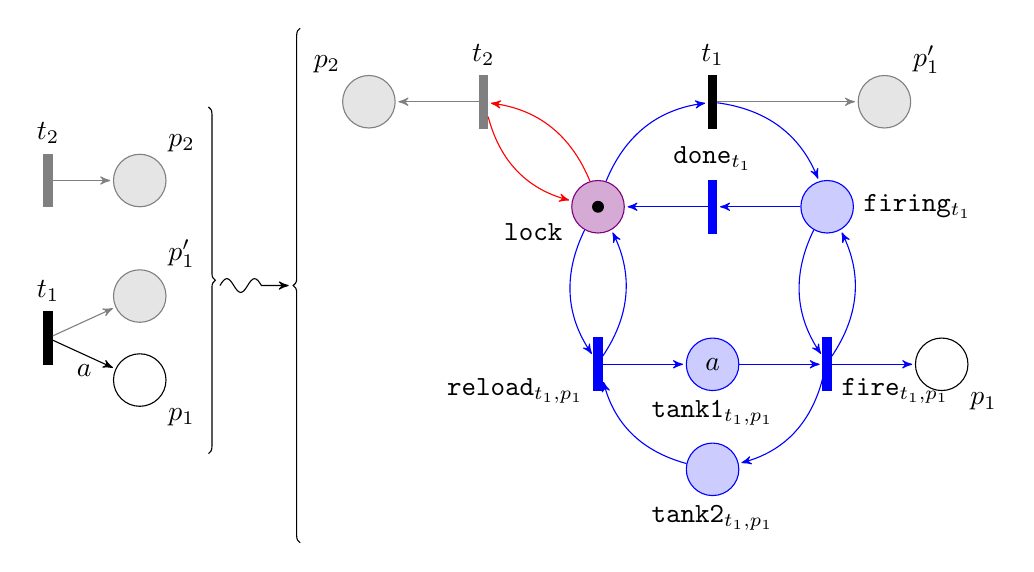
\begin{tikzpicture}[auto,x=0.12\linewidth,y=0.11\linewidth,
  silentp/.style={draw=blue,fill=blue!20},
  silentt/.style={draw=blue,fill=blue},
  silente/.style={draw=blue},
  parame/.style={},
  otherp/.style={draw=black!50,fill=black!10},
  othert/.style={draw=black!50,fill=black!50},
  othere/.style={draw=black!50},
  addede/.style={draw=red}
  ]
  \node [place,fill=blue!50!red!33,draw=blue!50!red] (l) [label=195:\texttt{lock},tokens=1]   at (1,3) {};
  \node [place,silentp] (f) [label=0:\texttt{firing}$_{t_1}$] at (3,3) {};
  \node [place,silentp] (t2) [label=270:\texttt{tank2}$_{t_1,p_1}$]  at (2,0.5) {};
  \node [place,silentp] (t1) [label=270:\texttt{tank1}$_{t_1,p_1}$]  at (2,1.5) {$a$};
  \node [place] (p1) [label=315:$p_1$]      at (4,1.5) {};
  \node [place,otherp] (p1p) [label=45:$p'_1$] at (3.5,4) {};
  \node [place,otherp] (p2)  [label=135:$p_2$] at (-1,4) {};

  \node [transition] (T1) [label=${t_1}$] at (2,4) {}
    edge [pre,  bend right, silente] (l)
    edge [post, bend left,  silente] (f)
    edge [post, othere]              (p1p);
  \node [transition,silentt] (D) [label=\texttt{done}$_{t_1}$] at (2,3) {}
    edge [pre,  silente]             (f)
    edge [post, silente]             (l);
  \node [transition,silentt] (R) [label=225:\texttt{reload}$_{t_1,p_1}$] at (1,1.5) {}
    edge [pre,  bend right, silente] (t2)
    edge [pre,  bend left,  silente] (l)
    edge [post, silente]             (t1)
    edge [post, bend right, silente] (l);
  \node [transition,silentt] (F) [label=315:\texttt{fire}$_{t_1,p_1}$] at (3,1.5) {}
    edge [pre,  bend left,  silente] (f)
    edge [pre,  silente]             (t1)
    edge [post, silente]             (p1)
    edge [post, bend right, silente] (f)
    edge [post, bend left,  silente] (t2);
  \node [transition,othert] (T2) [label=${t_2}$] at (0,4) {}
    edge [pre,  bend left,  addede] (l)
    edge [post, bend right, addede] (l)
    edge [post, othere] (p2);

  \begin{scope}[shift={(0,0.25)}]
    \node [place, label=45:$p'_1$, otherp] (pp1p) at (-3,1.9) {};
    \node [place, label=315:$p_1$]         (pp1)  at (-3,1.1) {};
    \node [place, label=45:$p_2$,  otherp] (pp2)  at (-3,3) {};

    \node [transition, label=$t_1$] at (-3.8,1.5) {}
      edge [post, othere] (pp1p)
      edge [post, parame] node[below] {$a$} (pp1);

    \node [transition, label=$t_2$, othert] at (-3.8,3) {}
      edge [post, othere] (pp2);
    
    \draw [decorate,decoration={brace,mirror}] (-2.4,0.4) -- (-2.4,3.7);
    \draw [->,decorate,decoration={coil,aspect=0}] (-2.3,2) -- (-1.7,2);
  \end{scope}
  \draw [decorate,decoration={brace}] (-1.6,-0.2) -- (-1.6,4.7);

\end{tikzpicture}

  \par
  \caption{From PostT-PPN to P-PPN}
  \label{fig:posttppn-to-pppn}
\end{figure}

\todo{We will see later that to establish that there is a simulation between two networks makes it possible to deduce many results.}

We can now construct for any PostT-PPN a P-PPN that simulates it.

Given a PostT-PPN $\namePPN[1] = \tuple{\places_1, \transitions_1, \parameters, \mar_{0,1}}$, create the new P-PPN $\namePPN[2] = \tuple{\places_2, \transitions_2, \parameters, \mar_{0,2}}$ like this.
Starting with an identical \ac{PPN}, first add a new place labelled \texttt{lock}, and, to all the transitions that does not have a parametrised output arc, add an input arc from, and an output one to \texttt{lock}.
Then, for all parametrised transition $t$, replace the parametrised output arcs by the silent subnet depicted in blue on figure~\ref{fig:posttppn-to-pppn}:
create a place \texttt{firing}$_t$ that will contains the ``lock token'' while simulating the firing of the parametrised transition, and a silent transition \texttt{done}$_t$ to release the lock,
then for all parameterized output arc to a place $p$, replace it by the places \texttt{tank1}$_{t,p}$, \texttt{tank2}$_{t,p}$ and the silent transitions \texttt{reload}$_{t,p}$, \texttt{fire}$_{t,p}$ as depicted.

Formally,
\begin{align*}
  \places_2 &= \places_1 \cup \{ \mathtt{lock} \}
    \cup \setComp{\mathtt{firing}_t}{\exists p \in \places_1 \text{ s.t. } \outm[\namePPN[1]][p,t] \in \parameters} \\
    &\qquad\cup \setComp{\mathtt{tank1}_{t,p}, \mathtt{tank2}_{t,p}}{\outm[\namePPN[1]][p,t] \in \parameters} \\
  \places_2 &= \bigcup \begin{cases}
      \places_1 \\
      \{ \mathtt{lock} \} \\
      \setComp{\mathtt{firing}_t}{\exists p \in \places_1 \text{ s.t. } \outm[\namePPN[1]][p,t] \in \parameters} \\
      \setComp{\mathtt{tank1}_{t,p}, \mathtt{tank2}_{t,p}}{\outm[\namePPN[1]][p,t] \in \parameters}
    \end{cases}\\
  \transitions_2 &= \bigcup \begin{cases}
      \transitions_1 \\
      \setComp{\mathtt{done}_t}{\exists p \in \places_1 \text{ s.t. } \outm[\namePPN[1]][p,t] \in \parameters} \\
      \setComp{\mathtt{fire}_{t,p}, \mathtt{reload}_{t,p}}{\outm[\namePPN[1]][p,t] \in \parameters}
    \end{cases}\\
  \inm[\namePPN[2]][p,t] &= \begin{cases}
      \inm[\namePPN[1]][p,t] &\text{ whenever } p \in \places_1 \wedge t \in \transitions_1 \\
      1 &\text{ whenever } p = \mathtt{lock}
          \wedge t \in \transitions_1 \cup \setComp{ \mathtt{reload}_{t',p'}}{t' \in \transitions_1, p' \in \places_1}\\
        &\quad\text{ or } p = \mathtt{firing}_{t'}
          \wedge t \in \{\mathtt{done}_{t'}\} \cup \setComp{\mathtt{fire}_{t',p'}}{p' \in \places_1} \\
        &\quad\text{ or } p = \mathtt{tank1}_{t',p'} \wedge t = \mathtt{fire}_{t',p'} \\
        &\quad\text{ or } p = \mathtt{tank2}_{t',p'} \wedge t = \mathtt{reload}_{t',p'} \\
      0 &\text{ otherwise }
    \end{cases} \\
  \outm[\namePPN[2]][p,t] &= \begin{cases}
      \outm[\namePPN[1]][p,t] &\text{ whenever } p \in \places_1 \wedge t \in \transitions_1 \wedge \outm[\namePPN[1]][p,t] \notin \parameters \\
      1 &\text{ whenever } p = \mathtt{lock}
          \wedge t \in \transitions_1 \wedge \nexists p' \text{ s.t. } \outm[\namePPN[1]][p',t] \in \parameters \\
        &\quad\text{ or } p = \mathtt{lock}
          \wedge t \in \setComp{\mathtt{done}_{t'}}{t' \in \transitions_1} \cup \setComp{\mathtt{reload}_{t',p'}}{t' \in \transitions_1, p' \in \places_1} \\
        &\quad\text{ or } p = \mathtt{firing}_{t'}
          \wedge t \in \{t'\} \cup \setComp{\mathtt{fire}_{t',p'}}{p' \in \places_1} \\
        &\quad\text{ or } p = \mathtt{tank1}_{t',p'} \wedge t = \mathtt{reload}_{t',p'} \\
        &\quad\text{ or } p = \mathtt{tank2}_{t',p'} \wedge t = \mathtt{fire}_{t',p'} \\
      0 &\text{ otherwise }
    \end{cases}\\
  \mar_{0,2}(p) &= \begin{cases}
      \mar_{0,1}(p)             &\text{ if } p \in \places_1 \\
      1                         &\text{ if } p = \mathtt{lock} \\
      \outm[\namePPN[1]][p',t'] &\text{ if } p = \mathtt{tank1}_{t',p'} \\
      0                         &\text{ otherwise }
    \end{cases}
\end{align*}
\todo{This break the formalism introduced at the benining}

This construction comes from \cite{David17}, to which we have added the uniqueness of the \texttt{lock} place for the whole network and its connection with all the transitions, even the non-parametrised ones.
This does not fundamentally change the properties of the newly built network, in that it also provides a simulation, but it reduces the size of its state tree.

\begin{lemm}
  For all valuation $v$ on $\parameters$, $v(\namePPN[2])$ weakly simulates $v(\namePPN[1])$.
\end{lemm}

\begin{proof}
  Let $\simeq$ be the weak simulation relation that witnesses it, \lang{i.e.} $\mar_{0,1} \simeq \mar_{0,2}$.
  This relation surely exists: we recursively show that it contains all the pairs $(\mar_1, \mar_2)$ such that
  \begin{align*}
    \mar_1 &\in \posts[\val]{\mar_{0,1}}\\
    \mar_2(p) &= \begin{cases}
        \mar_1(p) &\text{ if } p \in \places_1\\
        1         &\text{ if } p \text{ is } \mathtt{lock} \\
        \val[a]\text{, with $a$ the parameter from $t$ to $p'$ in $\namePPN[1]$} &\text{ if $p$ is }\mathtt{tank1}_{t,p'} \\
        0 &\text{ otherwise.}
      \end{cases}
  \end{align*}

  This holds for $(\mar_{0,1}, \mar_{0,2})$.

  Now, consider $\mar_1 \simeq \mar_2$.
  Thus, the induction hypothesis ensures that for all $\mar_1 \fire[{\val[{\namePPN[1]}]}]{t} \mar'_1$ the following sequence of transitions $\seqt$ is enabled in $\mar_2$:
  \begin{align*}
    \seqt = (t)
      &+ \outm[\namePPN[1]][p_{i_1},t] \cdot (\mathtt{fire}_{t,p_{i_1}})
       + \outm[\namePPN[1]][p_{i_2},t] \cdot (\mathtt{fire}_{t,p_{i_2}})
       + \dots \\
      &+ (\mathtt{done}_{t}) \\
      &+ \outm[\namePPN[1]][p_{i_1},t] \cdot (\mathtt{reload}_{t,p_{i_1}})
       + \outm[\namePPN[1]][p_{i_2},t] \cdot (\mathtt{reload}_{t,p_{i_2}})
       + \dots
  \end{align*}
  with $p_{i_1}, p_{i_2}, \dots$ the places $p_{i_j}$ of $\places_1$ such that $\outm[\namePPN[1]][p_{i_j}] \in \parameters$.
  Moreover, this sequence leads to a marking $\mar'_2$, $\mar_2 \fire[{\val[{\namePPN[2]}]}]{\seqt} \mar'_2$, for which the induction hypothesis holds.
  Thus $\mar'_1 \simeq \mar'_2$ and we can construct inductively the weak simulation relation.
  %First consider $v(\namePPN[1])$ and $v(\namePPN[1]')$ where $\namePPN[1]'$ is the network augmented by the \texttt{lock} place and its arcs from and to the non-parametrised transitions.
  %The simulation is obvious here: it contains all the pair of markings $(\mar_1, \mar_2)$ such that $\mar_1 \in \Post^*_v(\mar_{0,1})$ and
  %\[
  %  \mar_2(p) =
  %    \begin{cases}
  %      1 &\text{ if $p$ is \texttt{lock},} \\
  %      \mar_1(p) &\text{ otherwise.}
  %    \end{cases}
  %\]

  %Now consider $v(\namePPN[2])$ and focus on the parametrised transitions.
  %Each time an arc from $t$ to $p$ parametrised by $a$ ($\matO_{\namePPN[1]}(p)(t) = a$) is involved in a firing in $v(\namePPN[1])$, $v(a)$ tokens are created in $p$.
  %Regarding $v(\namePPN[2])$, the sequence $(t, \mathtt{fire}_{t,p}, \mathtt{done}_t, \mathtt{reload}_{t,p})$, where $\mathtt{fire}_{t,p}$ and $\mathtt{reload}_{t,p}$ are repeated $a$ times, creates $v(a)$ tokens in $p$ and reset the sub-net constructed for the simulation\todo{rewrite with regular notation}. Note that the rest of the network is not affected. Thus, monotonicity ensures that we have a weak simulation.
\end{proof}

Looking at the subnet in Figure~\ref{fig:posttppn-to-pppn},
one guesses that $\posts[\val({\namePPN[2]})]{\mar_{0,2}}$ does not contain “many” markings that are not involved in the weak simulation.
Indeed, by unfolding the transition relation on the created subnet for $\outm[\namePPN[1]][p,t] = a$, one can observe that the reachable markings when $t$ is fired only once are of the form:
\begin{align}
  \label{eqn:widget-reachable-markings}
  \mar_2(p') =
  \begin{cases}
    l   &\text{ if } p' \text{ is } \mathtt{lock}, \\
    f   &\text{ if } p' \text{ is } \mathtt{firing}_t, \\
    a_1 &\text{ if } p' \text{ is } \mathtt{tank1}_{t,p}, \\
    a_2 &\text{ if } p' \text{ is } \mathtt{tank2}_{t,p}, \\
    a_3 &\text{ if } p' \text{ is } p
  \end{cases}
  \text{\qquad with }
  \left\{
    \begin{aligned}
      l + f &= 1 \\
      a_1 + a_2 &= \val[a] \\
      a_3 \leq a_1 &\leq \val[a]
    \end{aligned}
  \right.
\end{align}

Thus, for all reachable marking $\mar_2 \in \Post^*_{v(\namePPN[2])}(\mar_{0,2})$ of \namePPN[2] there exists a reachable marking $\mar_1 \in \Post^*_{v(\namePPN[1])}(\mar_{0,1})$ of \namePPN[1] that ``covers'' it for all the common places: $\forall p \in \places_1, \mar_1(p) \geq \mar_2(p)$.
Actually, \namePPN[1] also simulates \namePPN[2].
(\namePPN[1] and \namePPN[2] are said to be \emph{weakly co-similar}.)

\begin{lemm}
  For all valuation $v$ on $\parameters$, $v(\namePPN[1])$ weakly simulates $v(\namePPN[2])$.
\end{lemm}

\begin{proof}
  We inductively create the weak simulation by keeping the following invariant:
  \( \mar_2 \simeq \mar_1 \Rightarrow \forall p \in \places_1, \mar_2(p) \geq \mar_1(p) \).
  Note that this property ensures that any visible transition enabled in $\mar_2$ is enabled in $\mar_1$.
  
  This holds for $(\mar_{0,2}, \mar_{0,1})$.

  Given a pair $\mar_2 \simeq \mar_1$ of the weak simulation, for all $\mar'_2$ given by
  $\mar_2 \fire[{\val(\namePPN[2])}]{t} \mar'_2$
  we add into the relation the pair $(\mar'_2, \mar'_1)$ where
  \begin{itemize}
    \item $\mar'_1$ is given by $\mar_1 \fire[{\val(\namePPN[1])}]{t} \mar'_1$ if $t \in \transitions_1$,
    \item $\mar'_1$ is $\mar_1$ otherwise, \lang{i.e.} if the $t$ is silent.
  \end{itemize}

  Indeed, if $t \in \transitions_1$, strong monotonicity of \ac{PN} ensures that the induction hypothesis holds for $(\mar'_2, \mar'_1)$.
  On the other hand, if $t$ is silent, either it is a transition $\mathtt{done}_{t'}$ or $\mathtt{reload}_{t',p'}$ and they do not change any place $p \in \places_1$; either it is a $\mathtt{fire}_{t',p'}$ transition and it adds a token in $p' \in \places_1$.
  However, $\mathtt{fire}_{t',p'}$ may be firered at most $\val[{\outm[{\namePPN[1]}]}]$ times each time $t'$ is fired once.
  (You can refer to~\cref{eqn:widget-reachable-markings} for more details.)
  This ensures that the induction hypothesis holds.
  %For all $\mar_{0,2} \fire[{\val(\namePPN[2])}]{t} \mar_{1,2}$, there exists $\mar_{1,1}$ such that $\mar_{0,1} \fire[{v(\namePPN[1])}]{t} \mar_{1,1}$.
  %After firing this first transition, either the transition was a non-parametrized one and we can repeat the operation, or it was parametrized and the lock disables the observable transitions until $\mathtt{done}_t$ has been fired.
  %In the latter case, any firable sequence ending with $\mathtt{done}_t$ is silent and produces a marking $\mar'_{1,2}$ covered by $\mar_{1,1}$.
  %Thus, by monotonicity and thanks to the lock, we know that once $\mathtt{done}_t$ has been fired, all the transitions enabled in $\mar'_{1,2}$ in \namePPN[2] are enabled in $\mar_{1,1}$ in \namePPN[1], except for some \texttt{reload} ones whose the effect is restricted to the \texttt{tank} places.
  %This can therefore be repeated and provides us with the desired weak-simulation.
\end{proof}

\paragraph{From P-PPN to PostT-PPN}

\subsection{Karp and Miller algorithm for \Ecov on PostT-\ac{PPN}}

The adaptation of the Karp and Miller algorithm to solve the \Ecov problem on PostT-\acp{PPN} is the result of one key observation.
In a PostT-\ac{PPN}, a place may contains an arbitrary large number of tokens either because of the presence of a self-covering increasing sequence, as in a plain \ac{PN}, or because of an arbitrary large valuation.
In the latter case, the place is not necessary \emph{unbounded}, that is to say, once a valuation is given, the number of tokens the place may contains may be bounded, even if the bound is arbitrary large due to the arbitrary large values of the valuation.
This is the case for place $p_1$ in the net shown in \cref{fig:postt-ppn-bound}: obviously it can contain $\val(\param)$ tokens, whose value may be arbitrarily high; but the place is bounded to this value.
The number of tokens in place $p_2$, on the contrary, is not bounded.

\begin{figure}[htbp]
  \centering
  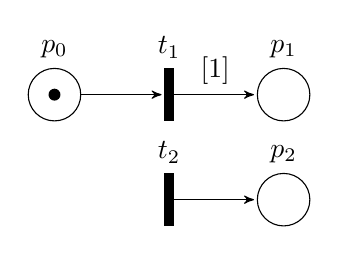
\begin{tikzpicture}[auto,x=0.12\linewidth,y=0.11\linewidth]
  \node [place,tokens=1] (p0) [label=$p_0$] at (-1,1) {};
  \node [place] (p1) [label=$p_1$] at (1,1) {};
  \node [place] (p2) [label=$p_2$] at (1,0) {};

  \node [transition] (t1) [label=$t_1$] at (0,1) {}
    edge [post] node [auto] {$\param[1]$} (p1)
    edge [pre] (p0);
  \node [transition] (t2) [label=$t_2$] at (0,0) {}
    edge [post] (p2);
\end{tikzpicture}

  \par
  \caption{An initialized PostT-\ac{PPN}}
  \label{fig:postt-ppn-bound}
\end{figure}

The adaptation of the Karp and Miller algorithm is therefore mainly the addition of a way to distinguish between these two cases.
It is done by introducing a new value allowed in the markings, noted $*$ and such that $* \notin \naturals$, $* \neq \omega$, and $\forall c \in \naturals$, we have:
\begin{itemize}
  \item $c < * < \omega$,
  \item $* - c = *$,
  \item $* + c = *$,
  \item $\omega - * = \omega$, and
  \item $\omega + * = \omega$.
\end{itemize}

For our purpose, we add: \todo{or not?}
\begin{itemize}
  \item $* + * = *$, and
  \item $\omega + \omega = \omega$.
\end{itemize}

$*$ being defined, the propagation of the $*$ still have to be ensured in the cases where all the input places of a transition are marked by a $*$, even if the output of the transition is not a parameter.
This is done by adapting the acceleration function.
This new acceleration function, $\Acc$, distinguishes three cases.
Given a marking to accelerate $\mar$ with the set $S$ of markings as the base of the acceleration,
the values of the different places of the accelerated marking are determined as follows:
\[
  \Acc(\mar, S)(p) =
  \begin{cases}
    \omega & \text{if } \exists \marp \in S : \marp \prec \mar
      \text{ and } \marp(p) < \mar(p) \\
      &\phantom{\text{if } \exists \marp \in S :}\text{ and }
        \forall p' \in \places, \mar'(p') \neq \omega:
        \effect{\mpath{\mar'}{\mar}}(p') \geq 0
        % Je pense que cette dernière condition est impliquée par la première
        % STOP HERE
  \end{cases}
\]
\todo{introduce \textbackslash mpath}
\begin{itemize}
  \item Either there exists $\marp \in S$ such that $\marp \fire{\sigma} \mar$, $\marp \prec \mar$, and for all place $p$ such that $\marp(p) \neq \omega$ we have $\effect{\sigma}(p) \geq 0$.\\
    This case corresponds to the classic acceleration and
    if $\marp(p) < \mar(p)$
    we have:
    \[
      \Acc(\mar, S)(p) = \omega
    \]
\item Or these first conditions does not hold but there exists a marking $\marp \in S$ such that $\marp \fire{\sigma} \mar$, $\marp \prec \mar$, and for all place $p$ such that $\marp(p) \notin \{\omega, *\}$ we have $\effect{\sigma}(p) \geq 0$.\\
    This case handle the propagation of the $*$ mentioned above and
    if $\marp(p) < \mar(p)$
    we have:
    \[
      \Acc(\mar, S)(p) = *
    \]
  \item Or no one of the previous cases holds.
    In this case $\Acc(\mar, S)(p) = \mar(p)$.
\end{itemize}

Intuitively, the second case formalise the idea that one can remove some tokens from a place with $*$ tokens without being an issue for the existence of a valuation that allows to cover a given marking.

Keeping in mind that we are looking for the existence of a valuation, as large as it may be, that allows to cover a (set of) marking(s) of the \ac{PPN} \namePPN, one can now perform the Karp and Miller algorithm, with the adapted acceleration function, on the plain \ac{PN} $v(\namePPN)$ where $v$ is the $*$-valuation that maps every parameter to $*$.

\subsection{Karp and Miller algorithm for \Ucov on PreT-\ac{PPN}}

Here is a symmetrical situation.
The parameters are used to indicate the number of tokens required for transitions to fire, and we want to determine if a (set of) marking(s) is coverable for all the possible valuations of the parameters, as large as they may be.
Therefore, the adaptation of the Karp and Miller algorithm lies on considering that a transition with parametric input arcs is enabled if and only if the corresponding places are marked by $\omega$.
This ensure that the transition is regarded as enabled only if it may actually fire whatever the valuation.
The other direction of the implication holds too, that is to say that, if a transition has a parametric input arc whose the corresponding place is bounded, there exists a valuation that does not enable the transition.
Indeed, recall that all simultaneous unbounded places in a \ac{PN} appear marked by $\omega$ in at least one label of the Karp and Miller tree for this \ac{PN}.

% vim: set spell spelllang=en :

\section{Known results on class \ac{PN}}
%% Intro
We now present the results related to the coverability problem on the plain \acp{PN} that we think are the most interesting.
To introduce these results, we need some additional definitions.
They will be given for plain \acp{PN}, but most of them are naturally extended to \acp{PPN}.

%% Covering set informal
Given an initialized \ac{PN} \N, the \emph{covering set} of \N is the set of markings covered by at least one reachable marking of \N.
It is an over-approximation of the reachability set that is precise enough to solve the coverability problem, and is, therefore, interesting for our study.

%% Covering set formal
\begin{defi}[Covering set]
  Let $\N = \PTm$ be an initialized \ac{PN}.
  The \emph{covering set} $S$ of \N, noted $\Cover(\N)$, is the set $\{c \mid \exists c' \in \Post^*(\N) : c \preceq c' \}$.
\end{defi}

%% Covering set picture
\begin{figure}[htbp]
  \label{fig:reach-and-cover-example}
  \centering
  \subfloat[A \ac{PN} ($|P| = 2$)]{
    \label{fig:two-net}
    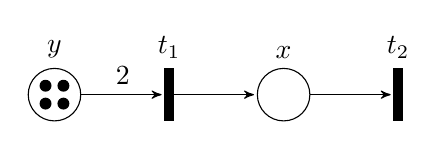
\begin{tikzpicture}[auto,x=0.12\linewidth,y=0.11\linewidth]
  \node [place, tokens=4] (y) [label=$y$] at (0,0) {};
  \node [place] (x) [label=$x$] at (2,0) {};

  \node [transition] (1) [label=$t_1$] at (1,0) [transition] {}
    edge [pre] node[midway, above] {2} (y)
    edge [post] (x);
  \node [transition] (2) [label=$t_2$] at (3,0) [transition] {}
    edge [pre] (x);
    %\node at (1.5,-0.75) {\label{2net} (1)\quad Un réseau de Petri ($|P| = 2$)};
\end{tikzpicture}


  }

  \subfloat[The reachable markings]{
    \label{fig:two-reach}
    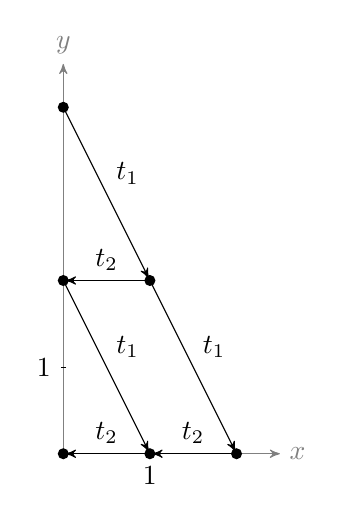
\begin{tikzpicture}[auto,x=1.1cm,y=1.1cm]
  \tikzset{
    >=stealth',
    axis/.style={thin, ->, line join=miter, color=gray},
    dot/.style={circle,fill=black,minimum size=4pt,inner sep=0pt,
          outer sep=-1pt}
  }
  \draw[axis,<->] (2.5,0) node(xline)[right] {$x$} -|
          (0,4.5) node(yline)[above] {$y$};

  \draw (1,1pt) -- (1,-1pt) node[anchor=north] {$1$};
  \draw (1pt,1) -- (-1pt,1) node[anchor=east] {$1$};

  \node[dot] (04) at (0,4) {};

  \node[dot] (12) at (1,2) {};
  \node[dot] (02) at (0,2) {};

  \node[dot] (20) at (2,0) {};
  \node[dot] (10) at (1,0) {};
  \node[dot] (00) at (0,0) {};

  \draw[->] (04) to node {$t_1$} (12);
  \draw[->] (12) to node {$t_1$} (20);
  \draw[->] (02) to node {$t_1$} (10);

  \draw[->] (12) to node[above] {$t_2$} (02);
  \draw[->] (20) to node[above] {$t_2$} (10);
  \draw[->] (10) to node[above] {$t_2$} (00);

  %\node at (1.2,-1) {\label{2reach} (2)\enspace Les marquages accessibles};
\end{tikzpicture}


  }\qquad
  \subfloat[The covering set]{
    \label{fig:two-cover}
    \begin{tikzpicture}[auto,x=1.1cm,y=1.1cm]
  \tikzset{
    >=stealth',
    axis/.style={thin, ->, line join=miter, color=gray},
    dot/.style={circle,fill=black,minimum size=4pt,inner sep=0pt,
          outer sep=-1pt}
  }

  \draw[axis,<->] (2.5,0) node(xline)[right] {$x$} -|
          (0,4.5) node(yline)[above] {$y$};

  \draw (1,1pt) -- (1,-1pt) node[anchor=north] {$1$};
  \draw (1pt,1) -- (-1pt,1) node[anchor=east] {$1$};

  \node[dot] at (0,4) {};

  \node[dot] at (1,2) {};
  \node[dot] at (0,2) {};

  \node[dot] at (2,0) {};
  \node[dot] at (1,0) {};
  \node[dot] at (0,0) {};

  \node[dot, color=black!60!white] at (0,3) {};
  \node[dot, color=black!60!white] at (0,1) {};
  \node[dot, color=black!60!white] at (1,1) {};

  %\node at (1.2,-1) {\label{2cover} (3)\enspace L'ensemble de couverture};
\end{tikzpicture}


  }
  \caption{Reachability and covering sets}
\end{figure}

The figure~\ref{fig:two-net} shows a marked \ac{PN} with two places.
One can therefore represents the markings as points on a plane.
The figure~\ref{fig:two-reach} shows the reachable markings in the form of an accessibility graph.
In~\ref{fig:two-cover} we see the covering set.

%% Unbounded places informal and self-covering sequence formal
Sometimes the number of tokens in a place is unbounded (\lang{c.f.} the place boundedness problem).
In a plain \ac{PN}, this is due to the existence of an increasing self-covering sequence.
\begin{defi}[Self-covering sequence]
  Given an initialized \ac{PN} $\N = \PTm$,
  a self-covering sequence is a sequence of the form:
  \(
    \mari \fire{\rho} \mar_i \fire{\sigma} \mar_j
  \),
  with $\rho$ and $\sigma$ two sequences of transitions of $T$
  and with $\mar_i \preceq \mar_j$.
\end{defi}

Note that, since $\mar_i \preceq \mar_j$, $\sigma$ is firable from $\mar_j$.
In addition, the monotonicity of \acp{PN} ensures that, with $\marp_j$ given by $\mar_j \fire{\sigma} \marp_j$, we have $\mar_j \preceq \marp_j$.
Thus, we see that it is a sufficient condition for the \emph{non-termination} of the system (the system may be able to fire transitions infinitely often).
In fact, because $\preceq$ is a well quasi-order (Lemma~\ref{lemm:wqo}), one can find in any infinite sequence $\mari \fire{} \mar_1 \fire{} \dots$ two markings $\mar_i$ and $\mar_j$ such that $\mar_i \preceq \mar_j$. \todo{take proof from mini-memoir.}
Therefore, any infinite sequence is self-covering, and the existence of such a sequence is also necessary for the non-termination of the system.

%% Increasing self-covering sequence formal
\begin{defi}[Increasing self-covering sequence]
  Given an initialized \ac{PN} $\N = \PTm$,
  an increasing self-covering sequence is a sequence of the form:
  \(
    \mari \fire{\rho} \mar_i \fire{\sigma} \mar_j
  \),
  with $\rho$ and $\sigma$ two sequences of transitions of $T$
  and with $\mar_i \prec \mar_j$.
\end{defi}

Let $Q \subseteq P$ be the set of places $Q = \{q \in P \mid \mar_i(q) < \mar_j(q)\}$.
$Q \neq \emptyset$ since $\mar_i \prec \mar_j$.

With a reasoning similar to the one above, we see that having such a sequence ensures that one can reach a marking $\marp_j$ given by $\mar_j \fire{\sigma} \marp_j$ such that $\mar_j \prec \marp_j$.
Because of the constant effect of transitions, we know that $\forall q \in Q : \mar_j(q) < \marp_j(q)$.
The unboundedness of the places in $Q$ follows.
\cite{David17} provides a complete proof.
\todo{A more formal proof that the existence of an increasing self-covering sequence is a necessary and sufficient condition for unboundedness on places is either to be done here or to be referenced.}

%% omark informal
An \omark is a way to represent a set of markings which have the same number of tokens in some places, and may have any number of tokens, potentially an infinity, in the other places.

%% omark formal
\begin{defi}[\omark]
  We define $\omega$ to be such that:
  $\omega \notin \mathbb{N}$
  and for any constant $c \in \mathbb{N}$:
  \begin{itemize}
    \item $c \leq \omega$
    \item $\omega + c = \omega$
    \item $\omega - c = \omega$
  \end{itemize}

  \emph{An \omark} \mar over a set of places $P$ is a function $\mar : P \mapsto \mathbb{N} \cup \{\omega\}$ that associates $\mar(p)$ tokens to each place $p \in P$.

  With $\mathbb{P}$ a set of parameters, $\omega \notin \mathbb{P}$,
  \emph{a parametric \omark} \mar over a set of places $P$ is a function $\mar : P \mapsto \mathbb{N} \cup \mathbb{P} \cup \{\omega\}$ that associates $\mar(p)$ tokens to each place $p \in P$.
\end{defi}

Note that an \omark \mar is a parametric \omark where $\mar(p) \in \mathbb{N} \cup \{\omega\}$ for all places $p \in P$.
Similarly, a parametric marking \mar is a parametric \omark where $\mar(p) \neq \omega$ for all places $p \in P$.
As for parametric markings, we often refer to a parametric \omark simply as \omark.

Given an \omark \mar, $\Omega(\mar) \subseteq P$ is the set of place $p$ such that $\mar(p) = \omega$, sometimes referred as \emph{\oplaces of \mar}. $P \setminus \Omega(\mar)$ is the set of \emph{\noplaces of \mar}.

%% Coverability set informal
\acp{PN} with unbounded places have an infinite reachability set.
So the covering set is also infinite.
\emph{Coverability sets} are useful to give a finite representation of the covering set thanks to \omark.
%%
In order to define them formally, we need to know about the maximal markings and the upward and downward closure of a set of markings.

%% Max markings informal
The maximal elements of a set are the markings that are not covered by any other marking of the set.
%% Max markings formal
\begin{defi}[Maximal markings]
  Given a set of markings $S$, the set of maximal elements of $S$ is
  $\Max(S) = \{ \mar \in S \mid \nexists \marp \in S \text{ s.t. } \mar \prec \marp \}$.
\end{defi}

%% Closure formal
\begin{defi}[Upward- and downward-closure on markings]
  Let $S \subseteq \mathbb{N}^{|P|}$ be a set of markings on the places $P$:
  \begin{itemize}
    \item The \emph{upward-closure} of $S$, noted $\upc(S)$, is the set
      $\{\mar \in \mathbb{N}^{|P|} \mid \exists \marp \in S : \marp \preceq \mar\}$,
    \item The \emph{downward-closure} of $S$, noted $\downc(S)$, is the set
      $\{\mar \in \mathbb{N}^{|P|} \mid \exists \marp \in S : \mar \preceq \marp\}$.
  \end{itemize}
  The closure of a marking \mar is the closure of the singleton $\{\mar\}$.
\end{defi}

%% Up closure example
For instance, with $\mar = (1, 2, 3)$, we have that its upward-closure is $\upc(\mar) = \{(i, j, k) \mid i \geq 1, j \geq 2, k \geq 3\}$.

%% Closed set formal
\begin{defi}[Upward- and downward-closed set of markings]
  A set $S$ of markings is said \emph{upward-closed} if $S = \upc(S)$.
  It is said \emph{downward-closed} if $S = \downc(S)$.
\end{defi}

%% Coverability set formal
\begin{defi}[Coverability set \citep{Finkel87,Finkel90}]
  Given an initialized \ac{PN} $\N = \PTm$, a \emph{coverability set} $S$ of \N is a set of markings such that $\downc(S) = \downc(\Post^*(\mari))$.
\end{defi}

%% Usefulness of coverability sets and omarks
Notice that, since $\downc(\mar)$ exists and is unique for all \omark \mar, an \omark may always stands for one and only one downward closed set.
Symmetrically, it is known that any downward closed set may be represented by a finite set of \omarks \citep{Geeraerts06}. \todo{Indeed...}

In particular, finite coverability sets may effectively represent, thanks to \omarks, any covering set:
Having an \omark \mar in a coverability set $S$ of $\N$ denotes that for all marking $\mar_1$ such that $\mar_1(p) = \mar(p) \forall p \in \{p \mid \mar(p) \neq \omega\}$, there exists a marking $\mar_2$ in the reachability set of \N such that $\mar_1 \prec \mar_2$.
\todo{We prove it by giving a minimal coverability set for any covering set.}

%% Max markings and minimal coverability set informal.
Indeed, the set of maximal reachable markings of \N exists, is finite and forms a minimal coverability set.

%% Max markings and minimal coverability set formal.
\[\downc(\Max(\Post^*(\mari))) = \downc(\Post^*(\mari))\]
\[\forall S \text{ such that } \downc(S) = \downc(\Post^*(\mari))\text{, we have } |S| \geq |\Max(\Post^*(\mari))|\]

Moreover, for any set of markings $S$ over a finite set of places $P$, the set of maximal markings of $S$ exists, is finite and is such that $\downc(\Max(S)) = \downc(S)$.

\todo{Lemme: For any downward-closed set S of markings, the downward-closure of the set of maximal markings of S is S}

\todo{Proof: the existence of a finite set of maximal elements}
It is straightforward to extend the proof to any downward-closed set.

%% coverability problem 2 formal
It is worth noticing that, in the context of \acp{PN}, the coverability problem for a set of markings $S$ may be defined as follows:
\begin{defi}[Coverability problem]
  \label{defi:upclocovprblm}
  Given a \ac{PN} \N and an upward-closed set $U = \upc(S)$ of markings of \N, determine whether $\Post^*(\mari) \cap U = \emptyset$.
\end{defi}

An upward closed set is always infinite.
It can be effectively represented through its unique set of minimal elements whose it is the upward closure:
\begin{lemm}
  For all upward-closed set $U \subseteq \mathbb{N}^{|P|}$, its set of minimal element $\Min(U) = \{\mar \in U \mid \nexists \marp \in U : \marp \prec \mar\}$ is such that $\upc(\Min(U)) = U$.
\end{lemm}

The following lemma ensure that this set is finite:
\begin{lemm}[Dickson's lemma]
  For all $c \in \mathbb{N}$, every set of $c$-tuples of natural numbers have finitely many minimal elements.
\end{lemm}
This result may easily be extended to $c$-tuples of values from any ordered countable set.

Moreover, this representation is effective in the sense that the set may be manipulated through it.
\cite{Ganty09} gives a way to perform the operations on upward closed sets through their minimal elements.

\subsection{A general backward algorithm $\back$}
\label{sec:backward-algorithm}

There exists a simple way to solve the coverability problem for all the examples of \acp{WSTS} above mentioned.
This algorithm was introduced by Abdulla \lang{et al.} \citep{Abdulla96}.
It is close of the one introduced earlier in \cite{Finkel90}.
%Even if we do not see how to use it in the context of \ac{PPN}, we mention it here because it helps to grasp, by comparison with the Karp and Miller algorithm presented in the following section, where does lie the difficulties of the coverability problem.

Relying on the definition~\ref{defi:upclocovprblm} of the coverability problem, given an upward-closed set of markings $U$, the algorithm computes $\Pre^*(U)$ by iterating the $\Pre$ operator.
\todo{The termination and correction of the algorithm were proven in cite{Abdulla96}. (check it)}
The termination is ensured by the existence of a fixed point in the sequence of upward closed set of markings $(R_i)_{i \geq 0}$:
\begin{gather*}
  R_0 = U \\
  \forall i > 0 : R_i = R_{i-1} \cup \Pre(R_{i-1})
\end{gather*}
When this fixed point is reached, we have $\Pre^*(U)$.
If $\mari \in \Pre^*(U)$, one can conclude positively.
Otherwise, the result is negative.
We call this algorithm $\back$.

This approach is elegant and general, but often inefficient in practice.
It is well-known that a forward exploration of the state of space (\lang{i.e.}, in this context, using $\Post$ instead of $\Pre$) is usually more efficient \citep{Henzinger98}.
We now present a forward algorithm, but whose the application is restricted to \ac{PN}.

\subsection{The Karp and Miller algorithm}

Although it was not originally designed for this purpose, the Karp and Miller algorithm \cite{Karp69} is a classical algorithm to compute a coverability set of an initialized \ac{PN}.
More precisely, it constructs a coverability tree and uses an acceleration function to systematically detect self-covering sequences, and thus ensures the termination.

\begin{defi}[Coverability tree]
  Given a \ac{PN} $\N = \PTm$, a coverability tree $\mathcal{T}$ of \N is a labelled tree $\mathcal{T} = \langle N, B, n_0, \Lambda\rangle$ where:
  \begin{itemize}
    \item $N$ is the set of nodes of the tree.%, is a set of \omark of \N such that $\downc(N) = \Cover(\N)$.
    \item $n_0 \in N$ is the root of the tree, \lang{i.e.} $\nexists n \in N$ such that $(n, n_0) \in B$.
    \item $\Lambda : N \mapsto (\mathbb{N} \cup \{\omega\})^{|P|}$ is a labelling function that associate to each node an \omark of \N.
    \item $B \subseteq N \times N$, the set of edges, is such that:
      \begin{itemize}
        \item with $(n_1, n_2) \in N^2$, if there exists an edge $(n_1, n_2) \in B$ then there exists a sequence $\sigma$ of transitions of $T$ such that $\Lambda(n_1) \fire{\sigma} \Lambda(n_2)$,
        \item for all node $n \in N \setminus \{n_0\}$, there exists a path from the root to $n$, that is, there exists a sequence of edges of $B$ of the form $((n_0, n_1), (n_1, n_2), \dots, (n_{i}, n))$, $i \geq 1$, and
        \item there are no cycles, that is, there are no sequences of edges of $B$ of the form $((n_1, n_2), (n_2, n_3), \dots, (n_i, n_1))$.
      \end{itemize}
  \end{itemize}
  and such that $\downc(\{\Lambda(n) \mid n \in N\}) = \Cover(\N)$.
\end{defi}

To keep $N$ finite, the Karp and Miller algorithm exploits the strong monotonicity of \acp{PN} to introduce \omark{}s through an \emph{acceleration function} $\KMAcc$.
This function takes a marking \mar to accelerate and a set of markings $S$ as a base for the acceleration and returns a marking $\mar_\omega$ such that:
\[
  \mar_\omega(p) =
  \begin{cases}
    \omega    &\text{if } \exists \marp \in S : \marp \prec \mar \text{ and } \marp(p) < \mar(p) \\
    \mar(p)  &\text{otherwise}
  \end{cases}
\]

The acceleration function is said to accelerate a marking if the first case holds for one or more place.
These places are said \emph{accelerated}.

We denote by $\treepath{n}$ the path in the tree from the root to $n$, that is the sequence of nodes from $n_0$ to $n$.
$\treepath{n}$ is called \emph{the branch to $n$} and the nodes of $\treepath{n}$ are the \emph{ancestors} of $n$.
$\treepath{m,n}$ is the sequence of nodes from $m$ to $n$.
%$\treepath{n}$ is the sequence of nodes from the path, $\treepathe{n}$ is the sequence of edges.

The algorithm constructs the tree $\mathcal{T}$ as follows:
The root $n_0$ of the tree is labelled with \mari.
A frontier $F$ is defined to be the set of unprocessed nodes of the tree and is initialised to $\{n_0\}$.
Then, while $F$ is non-empty, a node $n$ is chosen from $F$ to be processed:
(1) it is removed from $F$, and (2) if there is no node $n'$ in $\mathscr{T}_n$ such that $\Lambda(n) = \Lambda(n')$, then for all \omark $\mar \in \Post(\Lambda(n))$, (2.1) a node labelled with $\KMAcc(\mar, \mathscr{T}_n)$ is added to the frontier and (2.2) to the tree as a child of $n$.

The correctness and the termination of the algorithm lies on the strong monotonicity of \acp{PN}, and was proved by Karp and Miller in their work \cite{Karp69}.

%%%%%%%%%%%%%%

To prove that the Karp and Miller Tree $\mathcal{T}$ is a coverability tree of \N, we show
\begin{enumerate}
  \item \todo{} that one can construct a sequence from \mari to any marking \mar “covered by the tree” given a node $n$ such that $\mar \in \downc(\Lambda(n))$, and
  \item \todo{} that any marking $\mar \in \Post^*(\mari)$ is “covered by at least one node of the tree”.
\end{enumerate}

\todo{} Finally, we prove that $\mathcal{T}$ is finite and that the algorithm terminates.

Although very different in form, the proofs are based on those stated in \cite{Karp69}.

\begin{lemm}
  Given an initialized \ac{PN} $\N = \PTm$ and a node $n$ of its Karp and Miller tree $\mathcal{T} = \langle N, B, n_0, \Lambda\rangle$,
  for any marking $\mar \in \downc(\Lambda(n))$ there exists a sequence of transitions $\sigma \in T^*$ and a marking $\marp$ such that $\mari \fire{\sigma} \marp$ and $\mar \preceq \marp$.
\end{lemm}
\begin{proof}
  We show that there exists a function $\Sigma : \mathbb{N}^{|P|} \times N \mapsto T^* : \mar, n \rightarrow \sigma$ that, given a marking $\mar$ and a node $n$ such that $\mar \in \downc(\Lambda(n))$, gives such a sequence $\sigma$.

  For this purpose, we introduce some notations:
  \begin{itemize}
    \item we attach to the Karp and Miller tree $\mathcal{T}$ the mapping $\lambda : N \setminus \{n_0\} \mapsto T$ that gives for all node of the tree (but the root) the transition used to create it at step (2) of the Karp and Miller algorithm.

      By abuse of notation, we will note $\lambda((n_1, n_2, ..., n_m))$
      %with $n_i, i \in \{1, ..., m\}$ some nodes of $\mathcal{T}$
      with  $n_i \in N$
      the sequence $(\lambda(n_2), ..., \lambda(n_m))$.
    \item for any $n \in N \setminus \{n_0\}$, $\parent{n}$ is the direct ancestor, or \emph{parent}, of $n$ in $\mathcal{T}$, that is, the last but one node in $\treepath{n}$.
    \item given a sequence of nodes, for any node $n$ of the sequence but the last one, $\child{n}$ is the next node in the sequence.
    \item \todo{introduce operations on sequences: k.s, s1+s2}
  \end{itemize}

  Before we look at $\Sigma$, here is one key observation on the Karp and Miller tree:
  since the Karp and Miller algorithm never remove $\omega$s, we know that $\Omega(\Lambda(n)) \subseteq \Omega(\Lambda(\child{n}))$.
  Thus we have for any node $n \in N$ three disjoint sets of places whose the union is $P$:
  \begin{itemize}
    \item $\eta(n) = P \setminus \Omega(\Lambda(n))$ are the \noplaces of $\Lambda(n)$,
    \item $\zeta(n) = \Omega(\Lambda(\parent{n}))$ are the \oplaces that were already accelerated in $\Lambda(\parent{n})$, and
    \item $\alpha(n) = \Omega(\Lambda(n)) \setminus \Omega(\Lambda(\parent{n}))$ are the newly accelerated places.
  \end{itemize}


  Without loss of generality, we assume that $\mari$ does not map any place to $\omega$.

  We now recursively show that $\Sigma(\mar, n)$ exists for all such $\mar, n$ pair.

  If $n$ is the root of the Karp and Miller tree, \mar is covered by $\Lambda(n_0)$ and thus $\Sigma(n, \mar)$ is the empty sequence:
  \( \Sigma(n, \mar) = () \text{ whenever } n = n_0 \).
  This is the base case.
  We now present several simple cases for the induction step in order to easily introduce the general case.

  If $\Lambda(n)$ does not map any place to $\omega$, then,
  none of $\left\{\Lambda(n') \mid n' \in \treepath{n}\right\}$ do
  (since the Karp and Miller algorithm never removes $\omega$s)
  and \mar is covered by $\Lambda(n)$.
  Thus, the sequence comes directly from $\treepath{n}$.
  \( \Sigma(n, \mar) = \lambda(\treepath{n}) \text{ whenever } \Omega(\Lambda(n)) = \emptyset \).
  %Note that the previous case is a special case of this one.
  In a recursive way, this can be expressed as follows: $\Sigma(n, \mar) = \Sigma(\parent{n}, \Lambda(\parent{n})) + \lambda(n) \text{ whenever } \Omega(\Lambda(n)) = \emptyset$.
  %\( \Sigma(n, \mar) = \lambda(\treepath{n}) \text{ whenever } \nexists p \in P \text{ s.t. } \Lambda(n)(p) = \omega \)
  %\[ \Sigma(n, \mar) = \Sigma\big(P(n),\Lambda(P(n))\big) + (\lambda(n)) = \lambda(\treepath{n}) \text{ whenever } \nexists p \in P \text{ s.t. } \Lambda(n)(p) = \omega \]

  If $n$ is the first node of the branch labelled with a marking with places mapped to $\omega$,
  that is $\zeta(n) = \emptyset \wedge \alpha(n) \neq \emptyset$,
  we construct $\Sigma(n, \mar) = \sigma$ as follows.
  (Here are the ideas, we express them more precisely and in a recursive way right after.)\\
  First, consider the case where there exists exactly one \oplace $p$ in $\Lambda(n)$.
  This $\omega$ was introduced by $\KMAcc$ thanks to a node $n' \in \treepath{n}, \Lambda(n') \prec \Lambda(n)$.
  Thus $\lambda(\treepath{n',n})$ is an increasing self covering sequence
  and
  there exists some $k \in \mathbb{N}$ and $\marp \in \mathbb{N}^{|P|}$, $\mar \preceq \marp$
  such that
  $\sigma = \lambda(\treepath{n'}) + k \cdot \lambda(\treepath{n',n})$ and $\mari \fire{\sigma} \marp$. % with $\mar \preceq \marp$.
  More precisely, one can choose any $k$ that verifies $k \geq \left\lceil\frac{\mar(p) - \Lambda(n')(p)}{\Effect(\lambda(\treepath{n',n}))}\right\rceil$. %, but lower $k$ may also exists \todo{see notes +1+}.
  Note that $k > 0$.\\
  Second, if there exists many \oplaces $p_i$ in $\Lambda(n)$, one can compute $\sigma$ by considering the different $p_i$ one by one:
  We obtain for $p_1$ the sequence $\sigma_1 = \lambda(\treepath{n_1'}) + k_1 \cdot \lambda(\treepath{n_1',n})$ as above.
  Let $s_i$ be the sequence of nodes used to obtain $\sigma_i$, that is $s_1 = \treepath{n_1'} + k_1 \cdot \treepath{n_1',n}$.
  Now observe that
  the second $\omega$ was introduced thanks to a node $n_2$ that may appear many times in $s_1$ (it does whenever $n_2 \in \treepath{n_1',n}$ and $k_1 > 1$).
  This recursively extends to any $i \geq 2$.
  So, the construction of $\sigma_i$ is the same that for $\sigma_1$ except that we use $s_{i-1}$ instead of $\treepath{n}$ and that if $n_i'$ appears many times in $s_{i-1}$, we consider one of its occurrence. Note that the last one should produce the shortest sequence.%whenever there is many $n_i'$ in $\sigma_{i-1}$ we consider the last one of $\sigma_i$.
  \todo{illustration}

  Let us now express this in a more formal and recursive way.\\
  Since $\zeta(n) = \emptyset$, the previous case give us $\Sigma(\parent{n}, \Lambda(\parent{n}))$.
  We denote by $s_0$ the sequence of nodes used to obtain $\Sigma(\parent{n}, \Lambda(\parent{n}))$.
  Here this sequence is $\treepath{\parent{n}}$, but for the cases that follow, let's keep in mind that $s_0$ is the sequence of nodes used to obtain $\Sigma(\parent{n}, \mathit{previous\_marking})$, whatever $\mathit{previous\_marking}$ is.\\
  Each place $p_i, i \in \{1, 2, ..., I\}$ of $\alpha(n)$ is accelerated thanks to a node $n_i$.
  We give an order on this places such that, for $i \leq j$, $\treepath{n_i}$ is shorter or as long as $\treepath{n_j}$.
  This is to consider the longest self increasing covering sequences first and thus obtain the shortest sequence $\sigma$ \todo{to prove}.\\
  We compute the sequence of nodes $s$ such that $\sigma = \lambda(s) = \lambda(s_0 + (n) + s_I)$.
  $s_0 + (n)$ is the ``simple way'' to reach a marking $\downc(\Lambda(n))$ and whose the \noplaces have the values of those of $\Lambda(n)$.
  We compute shortest $s_I$ to have \marp, $\mar \preceq \marp$:
  \[
    s_i =
    \begin{cases}
      \left\lceil
        \frac{\mar(p_i) - \mari(p_i) - \Effect(\lambda(s_0+(n)))(p_i)}
            {\Effect(\lambda(\treepath{n_i,n}))}
      \right\rceil
      \cdot \treepath{n_i,n}
      &\text{ if } i = 1\\
      \\
      \max\left(0,
        \left\lceil
          \frac{\mar(p_i) - \mari(p_i) - \Effect(\lambda(s_0+(n)+s_{i-1}))(p_i)}
              {\Effect(\lambda(\treepath{n_i,n}))}
        \right\rceil
      \right)
      \cdot \treepath{n_i,n}
      &\text{ if } i \in \{2, ..., I\}\\
    \end{cases}
  \]

So we have $\Sigma(n, \mar) = \Sigma(\parent{n}, \Lambda(\parent{n})) + \lambda((n) + s_I)$ whenever $\zeta(n) = \emptyset \wedge \alpha(n) \neq \emptyset$.

  %Since the sequences $s_i$ thus obtained begin with $\treepath{n}$, $\Sigma(n , \mar)$ can be expressed in a recursive form, but it is more complicated than necessary to prove its existence.
  %\todo{see notes +1+}




  If $\Lambda(n)$ was not accelerated but some of its ancestors was (that is:
  %$\exists p \in P : \Lambda(n)(p) = \omega$ and $\nexists p' \in P \text{ such that } \Lambda(n)(p') = \omega \wedge \nexists n' \in \treepath{n}, n' \neq n, \Lambda(n')(p') = \omega$.
  %$\exists p \in P \text{ such that } \Lambda(n)(p) = \omega$ and for all such $p$, $\exists n' \in \treepath{n}, n' \neq n, \Lambda(n')(p) = \omega$)
  $\alpha(n) = \emptyset \wedge \zeta(n) \neq \emptyset$)
  then
  %since the Karp and Miller algorithm never removes $\omega$s,
  we know that its parent $\parent{n}$ is labelled with a marking ``having all the $\omega$s'' of $\Lambda(n)$:
  $\Omega(\Lambda(n)) = \Omega(\Lambda(\parent{n}))$.\\
  One can easily compute the lowest marking $\marpp$ in $\downc(\Lambda(\parent{n}))$ such that $\marpp \fire{\lambda(n)} \marp$ with $\mar \preceq \marpp$:
  \[
    \marpp(p) = \begin{cases}
      \Lambda(\parent{n})(p)
        &\text{ if } p \notin \Omega(\Lambda(\parent{n})) \\
      \max(\mar(p) - \Effect(\lambda(n))(p), I_{\lambda(t)}(p))
        &\text{ otherwise}
    \end{cases}
  \]

  %We show that there exists a marking $\marpp \in \downc(\Lambda(\parent{n}))$ such that
  %(1) $\lambda(n)$ is enabled in $\marpp$
  %and that
  %(2) $\marp$ given by $\marpp\fire{\lambda(n)}\marp$ is such that $\mar \preceq \marp$.\\
  %To define \marpp we use $\Lambda(\parent{n})$ and choose some values for the \oplaces:
  %We claim that any \marpp as follows holds.
  %\[
  %  \marpp(p) = \begin{cases}
  %    \Lambda(\parent{n})(p)
  %      &\text{ if } p \notin \Omega(\Lambda(\parent{n})) \\
  %    c \text{ with } c \geq \max(\mar(p) - \Effect(\lambda(n))(p), I_{\lambda(t)}(p))
  %      &\text{ otherwise}
  %  \end{cases}
  %\]
  Indeed, %(1)
  $\lambda(n)$ is enabled in $\marpp$:
  for the \noplaces $p$ of $\Lambda(\parent{n})$, the Karp and Miller algorithm ensures that $I_{\lambda(t)}(p) \leq \marpp(p)$;
  and for the \oplaces $p$ of $\Lambda(\parent{n})$, the chosen value is at least $I_{\lambda(t)}(p)$.\\
  Moreover, %(2)
  $\mar \preceq \marp$:
  for the \noplaces $p$ of $\Lambda(\parent{n})$, we have $\marp(p) = \marpp(p) + \Effect(\lambda(n))(p) = \Lambda(n)(p) \geq \mar(p)$ by choice of $n$ and \mar;
  and for the \oplaces $p$ of $\Lambda(\parent{n})$, we have $\marp(p) = \marpp(p) + \Effect(\lambda(n))(p) \geq \mar(p)$ by construction of $\marpp$.\\
  Thus, $\Sigma(n, \mar) = \Sigma(\parent{n}, \marpp) + \lambda(n)$
  whenever
  $\alpha(n) = \emptyset \wedge \zeta(n) \neq \emptyset$.
  %This allows to define $\Sigma(n, \mar)$ recursively up on the branch.

  %We first compute a marking $\marpp \in \downc(\Lambda(n''))$ such that $\lambda(\treepath{n'',n})$ is enabled in $\marpp$, then we show that $\marp$ given by $\marpp\fire{\lambda(\treepath{n'',n})}\marp$ is such that $\mar \preceq \marp$.\\
  %\[
  %  \marpp(p) =
  %  \begin{cases}
  %    \Lambda(n'')(p)
  %      &\text{ if } \Lambda(n'')(p) \neq w \\
  %    \mar(p) - \min(\Effect(\lambda(\treepath{n'',n})), \max\I(\lambda(n_i))
  %      &\text{ otherwise and if } \Effect(\lambda(\treepath{n'',n})) < 0
  %  \end{cases}

  %then we compute a marking \marpp


  %then we construct $\sigma$ recursively on the nodes of the branch.
  %The base case is the one treated above, where $\omega$ are first introduced.
  %Otherwise, one can define a marking $\marpp$ such that $\marpp(p) = \min(\mar(p), \Lambda(\parent{n})(p))$.
  %And so we have $\Sigma(\mar, n) = \Sigma(\marpp, \parent{n}) + (\lambda(n))$.

  \todo{Formally}

  Finally, let us consider the general case.
  On the basis of the reflections presented above, we obtain the following method:\\
  First compute


  Finally, let us consider the case where $\Lambda(n)$ may have newly accelerated places as well as others \oplaces.
  Actually, all the cases studied above are special cases of this one.
  Here, one can compute $\Sigma(n, \mar)$ by combining the different constructions above:
  First create a marking
  \[
    \marpp(p) = \begin{cases}
      \Lambda(\parent{n})(p)
        &\text{ if } p \notin \Omega(\Lambda(\parent{n})) \\
      \max(\mar(p) - \Effect(\lambda(n))(p), I_{\lambda(t)}(p))
        &\text{ otherwise}
    \end{cases}
  \]

  Then, we fix an order on the places $p_i \in \alpha(n), i \in \{1, 2,…\}$ such that the places accelerated thanks to a node $n_i$ nearer of the root of the tree are the first in $(p_1, p_2...)$.
  Compute $k_1 = $ \todo{} and for $i \neq 1, k_i = $\todo{}.
  Then, it is easy to see that $\Sigma(n, \mar) = \Sigma(\parent{n}, \marpp) + \lambda(n) + k_1 \dot \lambda(\treepath{n_1,n}) + k_2 \dot \lambda(\treepath{n_2,n}) + …$
\end{proof}

%%%%%%%%%%%%%%

The Karp and Miller tree has a lot of convenient properties that allow, among other, to answer the coverability problem as well as the simultaneous place unboundedness problem.

\begin{defi}[Simultaneous place unboundedness]
  Let \NPTm be a marked \ac{PN}.
  Given a set of place $Q \subseteq P$, \N is said $Q$-simultaneous unbounded if and only if for any $c \in \mathbb{N}$ there exists \mar such that $\mari \fire* \mar$ and $\forall p \in Q : \mar(p) \geq c$.
\end{defi}

Furthermore, the Karp and Miller algorithm can easily be adapted to some parametric problems \cite{David17}, as we will show in \autoref{sec:preliminaries-ppn}.

However, this tree, although finite, is often much larger than the minimal coverability set, and cannot be constructed in reasonable time.
As a consequence, many improvements were proposed, as well as other algorithms with different approaches.

\subsection{Geeraerts method}
\label{sec:eff}

This is usually called ``an efficient computation method of the coverability set of \acp{PN}''.
It was proposed in \cite{Geeraerts07thesis, Geeraerts07} as another approach to the computation of the coverability set.
It is not based on the Karp and Miller algorithm and is not an alternative to it in the sense that it does not allow to answer the same set of questions than the Karp and Miller tree answers.
However, this technique solves the coverability problem more efficiently in practice.

As in the Karp and Miller algorithm, an acceleration function exploits the strong monotonicity of \acp{PN} to allow termination.
But here, the acceleration of a marking is performed with only one marking as the base (instead of a set of marking).

To choose the base to use, the algorithm works on pair of \omarks.
These pairs allow to record a relationship between the markings.
More precisely, the algorithm constructs a pair of \omarks $(\mar_1, \mar_2)$ only if $\downc(\mar_2) \subseteq \downc(\Post^*(\mar_1))$.

To reduce the size of the set of pairs of \omarks, only the pairs where the difference (as defined below) between $\mar_1$ and $\mar_2$ is maximal are kept.
This will be the purpose of the order $\sqsubseteq$ we will define and it is justified by the intuitive idea that two more distant markings produce larger accelerations.
Therefore, if the algorithm builds a pair $(\mar_1, \mar_2)$, it can forget about any other ($\sqsubseteq$-comparable) pair whose the elements are closer because
\begin{itemize}
  \item by monotonicity, all potential successors of the elements of this pair will be covered by successors of $\mar_1$ or $\mar_2$, and
  \item any acceleration that can be created from this pair is covered by an acceleration one can build from $(\mar_1, \mar_2)$.
\end{itemize}

To describe the algorithm more formally, we will need the following definitions:

Given a pair of \omarks $(\mar_1, \mar_2)$, we define:
\begin{itemize}
  \item $\Postb((\mar_1, \mar_2)) = \{(\mar_1, \marp), (\mar_2, \marp) \mid \marp \in \Post(\mar_2)\}$,
  \item and, with $\mar_1 \prec \mar_2$, $\Accelb(\mar_1, \mar_2) = \{(\mar_2, \KMAcc(\{\mar_1\}, \mar_2))\}$.
    $\Accelb(\mar_1, \mar_2)$ is not defined whenever $\mar_1 \nprec \mar_2$,
\end{itemize}

With $R$ a set of pair of markings, we define:
\begin{itemize}
  \item $\Postb(R) = \bigcup_{(\mar_1, \mar_2) \in R} \Postb((\mar_1, \mar_2))$
  \item $\Accelb(R) = \bigcup_{(\mar_1, \mar_2) \in R}^{\mar_1 \prec \mar_2} \Accelb((\mar_1, \mar_2))$
  \item $\Flatten(R) = \{\mar \mid \exists \marp : (\marp, \mar) \in R\}$
\end{itemize}

The computation of the coverability set of the marked \ac{PN} $\NPTm$ lies on the sequence $\CovSeq(\N) = (V_i)_{i \geq 0}$ of pair of \omarks, where, for all marked \ac{PN} $\N$ we have:
\begin{gather*}
  V_0 = \{(\mari, \mari)\} \text{ and } \\
  \forall i \geq 1 : V_i = V_{i-1} \cup \Postb(V_{i-1}) \cup \Accelb(V_{i-1})
\end{gather*}

One can show that,
first, for all node $n$ of the Karp and Miller tree, there exists a value $k \geq 0$ of $i$ such that $\Lambda(n) \in \Flatten(V_k)$,
second, all the markings produced by $\Postb$ and $\Accelb$ are in the coverability set of \N.
\todo{Indeed...}

These two results lead to the following lemma:
\begin{lemm}[\cite{Geeraerts07}]
  Given a marked \ac{PN} \N such that $\CovSeq(\N) = (V_i)_{i \geq 0}$,
  there exists $k \geq 0$ such that for all $l \in \{0, ..., k-1\}$ we have that $\downc(\Flatten(V_l)) \subset \downc(\Flatten(V_{l+1}))$
  and for all $l \geq k : \downc(\Flatten(V_l)) = \Cover(\N)$.
\end{lemm}

Thus, the algorithm idea is to compute $\CovSeq$ until it stabilizes, \lang{i.e.} to the lowest $l$ such that $\downc(\Flatten(V_l)) = \downc(\Flatten(V_{l-1}))$ and to return $\downc(\Flatten(V_l))$.

To perform it efficiently, one can use a well-chosen order $\sqsubseteq$ on the pair of markings.
This order intents to sort the pairs of markings according to the distance in between, and is used to keep only ``the more distant'' pairs.
Let us denote by $\ominus$ the componentwise difference between two markings and to extend it to \omarks.
Formally, given two \omarks $\mar_1$ and $\mar_2$ on a set of places $P$, $(\mar_1 \ominus \mar_2)(p)$ is defined for all $p \in P$ as:
\[
  \begin{cases}
    \omega & \text{ whenever } \mar_1(p) = \omega \\
    -\omega & \text{ whenever } \mar_2(p) = \omega \text{ and } \mar_1(p) \neq \omega \\
    \mar_1(p) - \mar_2(p) & \text{ otherwise}
  \end{cases}
\]

Now we can define $\sqsubseteq$.
Given two pairs $(\mar_1, \mar_2)$ and $(\marp_1, \marp_2)$ of \omarks over a set of places $P$:
\[
  (\mar_1, \mar_2) \sqsubseteq (\marp_1, \marp_2) \Leftrightarrow
  \begin{cases}
    & \mar_1 \preceq \marp_1 \\
    \wedge & \mar_2 \preceq \marp_2 \\
    \wedge & \forall p \in P : (\mar_2 \ominus \mar_1)(p) \leq (\marp_2 \ominus \marp_1)(p)
  \end{cases}
\]

For a set of pair of \omarks $R$, $\Maxs(R) = \{ r \in R \mid \nexists r' \in R, r \sqsubseteq r'\}$ is the set of highest \omark of $R$ with respect to $\sqsubseteq$.

This order has properties \citep{Geeraerts07} that allows to keep the sets of markings of $\CovSeq$ small.
Thus, one can compute $\Cover(\N)$ of a \ac{PN} \NPTm by computing the sequence $(V_i)_{i \geq 0}$ defined below until $\downc(\Flatten(V_i)) = \downc(\Flatten(V_{i-1}))$.
\begin{gather*}
  V_0 = \{(\mari, \mari)\} \text{ and } \\
  \forall i \geq 1 : V_i = \Maxs(V_{i-1} \cup \Postb(V_{i-1}) \cup \Accelb(V_{i-1}))
\end{gather*}

At the end, we have that $\downc(\Flatten(V_i)) = \Cover(\N)$.

The correction and termination of the algorithm as well as useful properties of $\sqsubseteq$ can be found in \cite{Geeraerts07, Ganty09}.

\subsection{The \ac{EEC} algorithm}
\label{sec:eec}

\ac{EEC}, introduced in \cite{Geeraerts07thesis, Geeraerts06}, is an iterative algorithm that allows, among other, to solve the coverability problem for \ac{PN}.
We present it restricted to this context, but it may be used for a wide range of well-structured transitions systems, which \acp{PN} is part of, because it relies only on the monotonicity, and not on the strong monotonicity, of these models.

The idea is to compute and refine simultaneously an over- and an under-approximation of the covering set of the \ac{PN} until one or the other allows to conclude.

The under-approximation is computed as follows:
We define $(C_i)_{i \geq 0}$ to be the sequence of finite set of markings holding no more than $i$ tokens in each place (plus \mari):
\[
  \forall i \in \mathbb{N} : C_i = \{0, ..., i\}^{|P|} \cup \{\mari\}
\]
At step $i$, the algorithm computes $\Sous(\N, C_i)$ defined as the graph $\langle C_i, \mari, \sousrel \rangle$ which is the transition system induced by the \ac{PN} \N restricted to the markings of $C_i$, \lang{i.e.} $(\mar_1, \mar_2) \in \sousrel$ if, and only if, $\mar_1 \rightarrow \mar_2$.
The under-approximation sought is the set of markings reachable through $\sousrel$ from \mari and is denoted $\R(\Sous(\N, C_i))$.

At step $i$, the algorithm also uses $L_i$ from the sequence $(L_i)_{i \geq 0}$ of finite set of \omarks such that $L_i = \{0, ..., i, \omega \}^{|P|} \cup \{\mari\}$.
That is, $L_i$ contains all the markings with at most $i$ tokens in any place, or $\omega$ (plus \mari).
This set is used to construct the graph $\Sur(\N, C_i)$ defined as the graph $\langle L_i, \mari, \surrel \rangle$ where $(\mar_1, \mar_2) \in \surrel$ if, and only if:
\begin{itemize}
  \item either $\mar_1 \rightarrow \mar_2$,
  \item either $\mar_1 \rightarrow \marp_2, \marp_2 \notin L_i, \marp_2 \preceq \mar_2, \text{ and } \nexists \marpp_2 \in L_i \text{ such that } \marp_2 \prec \marpp_2 \prec \mar_2$.
\end{itemize}
In other words: if $\mar_2 \notin L_i$, it is replaced by the lowest marking of $L_i$ which over-approximate it.
Note that this is an \omark which exists and is unique. \todo{Indeed...}
Then the over-approximation is the set of markings of $L_i$ reachable through $\surrel$ from \mari. It is denoted $\R(\Sur(\N, L_i))$.

We can say that they are under- and over-approximations thanks to the following lemmata:
\begin{lemm}[Under-approximation \cite{Ganty09}]
  For all \ac{PN} \NPTm, for all upward-closed set $U \subseteq \mathbb{N}^{|P|}$, and for all $i \geq 0: \R(\Sous(\N,C_i)) \cap U \neq \emptyset \Rightarrow \Post^*(\mari) \cap U \neq \emptyset$.
\end{lemm}
\begin{lemm}[Over-approximation \cite{Ganty09}]
  For all \ac{PN} \NPTm, for all upward-closed set $U \subseteq \mathbb{N}^{|P|}$, and for all $i \geq 0: \downc(\R(\Sur(\N,L_i))) \cap U = \emptyset \Rightarrow \Post^*(\mari) \cap U = \emptyset$.
\end{lemm}

One can prove that one of the conditions mentioned in the lemmata will eventually happen.
This ensures the termination of the algorithm.

Indeed, let $S$ be the set of markings we want to cover and let $U$ be $\upc(S)$.
If $U$ is reachable, we will eventually get a $C_i$ that contains all the markings of a path from $\mari$ to $U$.
As this path will be present in $\Sous(\N, C_i)$, we will have that $\R(\Sous(\N,C_i)) \cap U \neq \emptyset$.\\
Symmetrically, let $j$ be such that $L_j$ contains the maximal elements of the covering set of \N.
Such a $j$ exists, and we have that $\downc(\R(\Sur(\N,L_j))) = \Cover(\N)$.
Thus, we know that, for a negative instance of the problem, $\downc(\R(\Sur(\N,L_i))) \cap U = \emptyset$ will eventually happen for an $i \leq j$.


\removed{A backward algorithm \citep{Finkel90, Abdulla96}}
%\subsection{A backward algorithm \citep{Finkel90, Abdulla96}}
%
%We will now present an algorithm to solve the coverability problem for a marking \mar of a \ac{PN} $\N = \PTm$.
%
%This algorithm was introduced by Abdulla \lang{et al.} \cite{Abdulla96} for well-structured transition systems, a more general class of models which includes \acp{PN}.
%It is close of the one introduced earlier in \cite{Finkel90}.
%
%Recall the definition for a marking of being coverable.
%\coverability*
%
%For convenience, we will use another equivalent definition.
%
%\begin{defi}[Coverability]
%  Given an initialized \ac{PN} \NPTm and an upward-closed set $U$, $U$ is said coverable if there exists a marking \marp such that $\marp \in U$ and $\mari \fire{*} \marp$.
%\end{defi}
%
%By choosing $\upc(\mar)$ as $U$, these two definitions set out the same instance of the coverability problem.
%With a set of markings considered in the first definition, $U$ may be the union of their upward-closure in the second.
%
%We say it is a backward algorithm in the sense that it is based on the computation of the set $\Pre^*(\mar)$ and answer by checking whether $\mari \in \Pre^*(\mar)$; unlike a forward approach which would have calculated the reachability set and conclude by checking whether \mar was in it. In other words, it computes all the configurations that can reach $U$ in any number of steps.
%
%The calculation is a fixed point algorithm that compute the increasing sequence, for the inclusion relation, of sets of markings: $(R_n)_{n \in \mathbb{N}}$, with $R_0 = U$ and $R_{n+1} = \Pre(R_n) \cup R_n$.
%Thus, $R_n$ is the set of markings from which there exists a sequence of at most $n$ transitions which may be fired and that cover $U$.
%Because, with $U$ an upward-closed set of markings, $\Pre(U)$ is upward-closed too%
%\footnote{This is due to the monotonicity of \acp{PN}, \todo{see for example cite\{someone\}}},
%and because the union of two upward-closed sets is an upward-closed set,
%$R_n$ is upward-closed for all $n$.
%
%\todo{summarize correctness and termination from \cite{Abdulla96}}

% vim: set spell spelllang=en :


\vspace*{0.5cm}
\chapter*{Conclusions}

The conclusions are to be written with care\index{Care}, because it will be sometimes the part that could convince a potential reader to read the whole document.

\appendix

\backmatter

\printindex % use makeindex to generate the index

\bibliographystyle{plain}

\bibliography{info} %use bibtex to generate the bibliography

\end{document}

% vim: set spell spelllang=en :
